\documentclass[preprint, 3p,
authoryear]{elsarticle} %review=doublespace preprint=single 5p=2 column
%%% Begin My package additions %%%%%%%%%%%%%%%%%%%

\usepackage[hyphens]{url}

  \journal{Transport Geography?} % Sets Journal name

\usepackage{graphicx}
%%%%%%%%%%%%%%%% end my additions to header

\usepackage[T1]{fontenc}
\usepackage{lmodern}
\usepackage{amssymb,amsmath}
% TODO: Currently lineno needs to be loaded after amsmath because of conflict
% https://github.com/latex-lineno/lineno/issues/5
\usepackage{lineno} % add
\usepackage{ifxetex,ifluatex}
\usepackage{fixltx2e} % provides \textsubscript
% use upquote if available, for straight quotes in verbatim environments
\IfFileExists{upquote.sty}{\usepackage{upquote}}{}
\ifnum 0\ifxetex 1\fi\ifluatex 1\fi=0 % if pdftex
  \usepackage[utf8]{inputenc}
\else % if luatex or xelatex
  \usepackage{fontspec}
  \ifxetex
    \usepackage{xltxtra,xunicode}
  \fi
  \defaultfontfeatures{Mapping=tex-text,Scale=MatchLowercase}
  \newcommand{\euro}{€}
\fi
% use microtype if available
\IfFileExists{microtype.sty}{\usepackage{microtype}}{}
\usepackage[]{natbib}
\bibliographystyle{plainnat}

\usepackage{graphicx}
\ifxetex
  \usepackage[setpagesize=false, % page size defined by xetex
              unicode=false, % unicode breaks when used with xetex
              xetex]{hyperref}
\else
  \usepackage[unicode=true]{hyperref}
\fi
\hypersetup{breaklinks=true,
            bookmarks=true,
            pdfauthor={},
            pdftitle={Leveraging GTFS to explore spatial gaps in transit supply with respect to social needs},
            colorlinks=false,
            urlcolor=blue,
            linkcolor=magenta,
            pdfborder={0 0 0}}

\setcounter{secnumdepth}{5}
% Pandoc toggle for numbering sections (defaults to be off)


% tightlist command for lists without linebreak
\providecommand{\tightlist}{%
  \setlength{\itemsep}{0pt}\setlength{\parskip}{0pt}}




\usepackage{subfig}
\usepackage{booktabs}
\usepackage{longtable}
\usepackage{array}
\usepackage{multirow}
\usepackage{wrapfig}
\usepackage{float}
\usepackage{colortbl}
\usepackage{pdflscape}
\usepackage{tabu}
\usepackage{threeparttable}
\usepackage{threeparttablex}
\usepackage[normalem]{ulem}
\usepackage{makecell}
\usepackage{xcolor}



\begin{document}


\begin{frontmatter}

  \title{Leveraging GTFS to explore spatial gaps in transit supply with
respect to social needs}
    \author[Public Transport Research Group (PTRG)]{James Reynolds%
  %
  \fnref{1}}
   \ead{james.reynolds@monash.edu} 
    \author[Public Transport Research Group (PTRG)]{Graham Currie%
  \corref{cor1}%
  \fnref{2}}
   \ead{graham.currie@monash.edu} 
    \author[Public Transport Research Group (PTRG)]{Yanda Qu%
  %
  \fnref{3}}
   \ead{yanda.qu@monash.edu} 
      \affiliation[Public Transport Research Group (PTRG)]{
    organization={Public Transport Research Group (PTRG), Institute of
Transport Studies, Department of Civil Engineering Engineering, Monash
University},addressline={Clayton
Campus},city={Melbourne},postcode={3800},state={Victoria},country={Australia},}
    \cortext[cor1]{Corresponding author}
    \fntext[1]{Research Fellow}
    \fntext[2]{Professor}
    \fntext[3]{PhD Student}
  
  \begin{abstract}
  This is the abstract.

  It consists of two paragraphs.
  \end{abstract}
    \begin{keyword}
    keyword1 \sep 
    keyword2
  \end{keyword}
  
 \end{frontmatter}

\section{Introduction}\label{introduction}

A motivation for providing a basic level of transit service is to enable
those who cannot otherwise drive themselves to have at least some
mobility and accessibility to activities and service beyond walking
distance \citep{Currie:2016aa}. Age, disability, socio-economic status,
lack of a driver's license or vehicle, or other factors might make
someone reliant on transit services for some or all of their travel.
Social-equity perspectives on transport policy-making, especially those
related to vertical equity and better supporting those who are
disadvantaged (c.f. \citet{Litman:2016aa}), might therefore suggest
providing at least some transit, and probably more than just a minimum,
to places that have the highest social need for transport.

\citet{Currie2003Hobart}, \citet{Currie2004Gap};
\citet{Currie2007Identifying}; \citet{currie2010identifying} developed
an approach for identifying spatial gaps in transit supply related to
social needs for transport. This was applied to a case study of
Melbourne in 2006 in \citet{Currie2007Identifying};
\citet{currie2010identifying}. However, there does not appear to have
been much further use or development of this approach. It is unclear
whether the spatial patterns identified in this previous research are
representative of transit supply and social needs in other places, or if
the situation in Melbourne has changed in the intervening years. This
may in part be because, until recently, transit schedule data was not
typically available in consistent, electronic formats, meaning that
assessing transit supply was a large task requiring data to be sourced,
cleaned and analysed for each individual transit operator.

Nowadays, however, more than 10,000 transit agencies publicly release
timetable data in the General Transit Feed Specification (GTFS) format
\citep{GTFS}. Such standardisation allows Google Maps and other online
platforms to provide transit-related outputs for any place with a GTFS
feed. It also facilitates data access and processing for research
purporsesx. However, tools for using GTFS data to examine spatial
patterns and gaps in transit supply with respect to social needs for
transport do not appear to be readily available. This gap, and the lack
of direct follow up to \citet{Currie2003Hobart}, \citet{Currie2004Gap},
\citet{Currie2007Identifying} and \citet{currie2010identifying}, provide
motivation for research.

The objectives of this research are: (1) to develop tools for
undertaking needs-gap analysis using GTFS datasets; and (2) to explore
whether the spatial pattern of gaps reported in
\citet{Currie2007Identifying} and \citet{currie2010identifying} are
consistent with current patterns. Research outcomes that are reported in
this paper include the development of a new R package (gtfssupplyindex)
that includes software tools for using the \citet{Currie2007Identifying}
and \citet{currie2010identifying} analysis approach, in particular the
calculation of transit Supply Index (SI) scores from GTFS datasets. Also
presented in this paper are results for Melbourne in 2016 and 2021,
matching the most recent censuses, which are compared to the 2006
analysis reported in \citet{currie2010identifying}\footnote{The wider
  programme of research includes examination of spatial gaps in other
  cities, so as to better understand whether patterns in Melbourne are
  representative of other places. However, this paper is limited to
  examining Melbourne in 2016 and 2021 only. Results for other cities
  will be reported elsewhere.}.

The remainder of this paper is structured as follows: the next section
outlines the research context. Section 3 describes the study
methodology, followed by presentation of results in Section 4 and
discussion in Section 5. Limitations of this study and directions for
future research are discussed in Section 6, which also includes a brief
conclusion

\section{Research context}\label{research-context}

There are many metrics available for assessing transit services.
Examples include: those in the Transit Cooperative Research Program
(TCRP) Report 88 (a guidebook for developing performance-measurement
systems \citep{Ryus:2003aa}); and those used across benchmarking
databases and programs such as by
\citet{Florida-Transit-Information-System:2018aa}, the
\citet{UITP:2015aa} and \citet{Imperial-College-London:2023aa}. The
Fielding Triangle \citep{FieldingGordonJ1987Mpts} provides a framework
for combining indicators of service inputs, outputs and consumption to
describe cost efficiency, cost effectiveness and service effectiveness.
More broadly: \citet{Litman:2003ab} and \citet{Litman:2016aa} discuss
some of the traffic, mobility, accessibility, social equity, strategic
planning and other rational decision-making-based perspectives
underlying many transport indicators; \citet{Reynolds:2017ah} extends
these into models of how institutionalism, incrementalism and other
public policy analysis concepts might apply to decision-making processes
relating to transit prioritization; \citet{GuzmanLuisA.2017Aeit}
developed a measure of accessibility in the context of policy
development and social equity for Latin American Bus Rapid Transit (BRT)
networks; and \citet{Creutzig2020streetspaceallocation} introduced
street space allocation metrics based around ten ethical principles.

Many such metrics, however, may be difficult to calculate, explain or
understand, especially for those who are not planners, engineers or
other technical specialists. Where pre-calculated transit metrics are
immediately available, such as on a website or other online platform, it
may not be possible to independently generate scores, for instance to
assess proposed system changes. Contrasting examples are provided by:

\begin{itemize}
\item
  Transit Scores \citep{WalkScore:2023tg}, which are readily available
  online for locations with a published GTFS feed. The meaning of the
  metric appears easy to explain, with the highest possible score of 100
  representing the sort of transit accessibility experienced in the
  center of New York. However, the Transit Score algorithm is secret,
  and scores cannot be calculated independently or generated for
  proposed changes to a network.
\item
  The Transit Capacity and Quality of Service Manual (TCQSM), which
  provides a wide range of metrics for measuring different aspects of a
  transit system. The TCQSM scores themselves appear easy to understand
  or explain, ranging from A (good) to F (bad), although there are a
  large number of metrics which may add to the complexity of using these
  in practice for communication with non-technical audiences (e.g.~for
  communication with the public, politicians or other stakeholders).
  TCQSM scores, however, can be calculated independently, given
  sufficient data.
\end{itemize}

The widespread availability of GTFS datasets in recent years has
facilitated the development of tools that apply one or a group of
metrics to many transit systems. The Transit Score website provides one
example. \citet{Wong:2013aa} provides another in reporting the
distribution of various TCQSM metrics across 50 USA transit operators.
Code used in the \citet{Wong:2013aa} analysis is available for those who
might wish to produce similar analysis for other locations or time
periods. Developing a similar code base, but for calculating metrics
associated with spatial gaps in transit supply with respect to social
needs, is the subject of this paper.

\subsection{The Transit Suppy Index}\label{the-transit-suppy-index}

A generalized form of the SI equation, adapted from
\citet{currie2010identifying}, is:

\[SI_{area, time} = \sum{\frac{Area_{Bn}}{Area_{area}}SL_{n, time}}\]

where:

\begin{itemize}
\item
  \(SI_{area, time}\) is the Supply Index for the area of interest and a
  given period of time;
\item
  \(Area_{Bn}\) is the buffer area for each stop (n) within the area of
  interest (in \citet{currie2010identifying} this was based on a radius
  of 400 metres for bus and tram stops, and 800 metres for railway
  stations);
\item
  \(Area_{area}\) is the area of the area of interest; and
\item
  \(SL_{n,time}\) is the number of transit arrivals for each stop for a
  given time period.
\end{itemize}

\begin{figure}
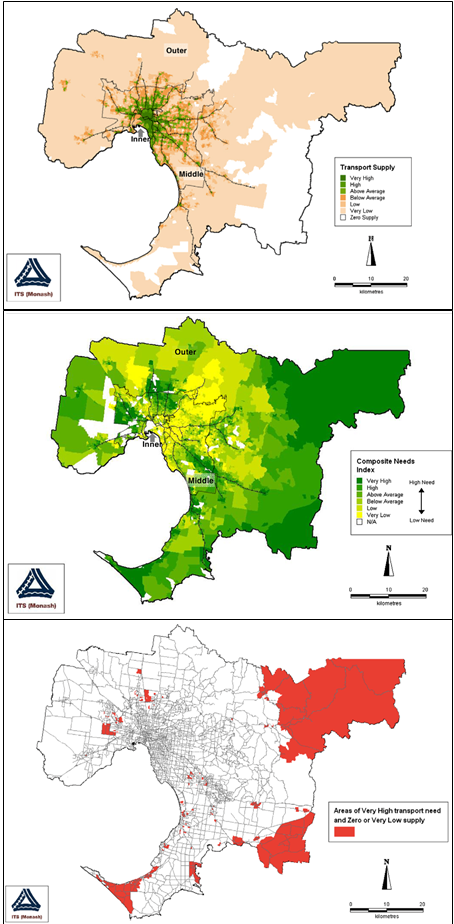
\includegraphics[width=0.9\linewidth]{graphics/Currie2010combined1} \caption{Melbourne 2006: Distribution of supply measure scores (top), needs (middle) and gaps (bottom), Source: Currie (2010)}\label{fig:Currie_map_SI}
\end{figure}

\citet{currie2010identifying} reported SI scores for Census Collection
Districts (CCDs) across Metropolitan Melbourne in 2006. These were used
to categorised service levels into seven groups, as shown in Figure
\ref{fig:Currie_map_SI} (top). General patterns were identified, being:
more transit supply in the inner and middle suburbs, and along passenger
railway lines; and outer areas tending to have very low SI scores or no
transit supply at all.

\subsection{Social need and needs-gap}\label{social-need-and-needs-gap}

As well as measuring transit supply, \citet{currie2010identifying}
assessed the social need for transport across Melbourne using: the
Australian Bureau of Statistics' (ABS') Index of Related Socio-Economic
Advantage/Disadvantage (IRSAD) and a transport needs index derived from
eight weighted indicators. The spatial distribution of this composite
social needs index, reproduced in Figure \ref{fig:Currie_map_SI}
(middle), showed that areas of above average, high and very high social
needs in 2006 were located in: some outer areas, particularly in the
east and south-east; and in some middle areas in the south-east, north
and west.

As the final step in the spatial needs-gap analysis,
\citet{currie2010identifying} identified areas with very high transport
needs, but very low or zero transit supply, as reproduced in Figure
\ref{fig:Currie_map_SI} (bottom). These areas were identified as being
those where service gaps might be of particular concern. Most of these
were located in outer parts of Melbourne in the north-east, south-east
and south, although there were also some pockets in the middle suburbs
in the west, north and south east. Overall,
\citet{currie2010identifying} found that ``8.2\% of Melbourne residents
have `very high' needs but `zero', `low' or `very low' public transport
supply.''

Using this methodology in transit planning was suggested as
``substantially more useful than the presentation of anecdotal evidence,
which is the most common means of identifying transport needs in local
transport studies throughout the world'' \citep{currie2010identifying}.
However, it does not appear that this approach has been widely adopted
in practice or by researchers. Our suspicion is that while the SI has a
relatively simple formula and requires only geographic and timetable
data to calculate, a lack of software tools to complete the analysis may
be partly why it has not been more widely adopted.

It is also unclear whether the patterns in Melbourne identified in
\citet{currie2010identifying} have changed since the 2006 analysis, or
if Melbourne is representative of other locations. Developing a software
tool to calculate SI tools from GTFS data, and using it to comparing
current conditions to the findings of \citet{currie2010identifying},
therefore, provides motivation for this research.

\section{Methodology}\label{methodology}

Case research approaches can be particularly useful research questions
are about `how' or `why', but when researchers do not have control of
events and so cannot use experimental approaches \citep{Yin2009aa}. In
this research study questions relate to (1) how to use GTFS data to
assess gaps between social needs and transit supply, and (2) how and why
spatial patterns might have changed since those reported for 2006 in
\citet{currie2010identifying}. There is no ability here to control
events related to spatial patterns of social needs and gaps in transit
supply, so a case research approach appears well suited to this study.

There is a need to addressing the ``duality criterion'' when using a
case research approach, this being the need of the research to be
seeking generalisable findings while at the same time being grounded in
the context of only a small number of cases
\citep{Denscombe2007aa, Ketokivi2014aa}. Here the approach taken has
been to develop a package of tools for calculating the SI from GTFS data
using the R programming language \citep{R-base}. Using these methods
addresses the duality criterion for the first research question, as the
developed software functions are generic. They are applicable to other
GTFS feeds, and could be used to analyse spatial gaps in transit supply
in other places (and by others), beyond the Melbourne case reported in
this paper. The recommendations of \citet{wickham2023r} informed the
package setup and development approach. Various existing packages and
code examples were relied upon including: the sf package \citep{R-sf}
for geospatial analysis; the tidyverse \citep{tidyverse2019}; gtfstools
\citep{R-gtfstools}; and tidytransit \citep{R-tidytransit}.

There are, however, limitations to the generalisability of the findings
of this research with respect to changes since 2006 and the patterns
reported in \citet{currie2010identifying}(research question 2).
\citet{Currie2007Identifying} and \citet{currie2010identifying} reported
results for Melbourne only. The \citet{Currie2003Hobart} and
\citet{Currie2004Gap} studies of Hobart and Adelaide used earlier
versions of the needs-gap assessment methodology, for which further
software tools have not been developed. While this study does seek to
findings about changes in spatial patterns of social need and transit
supply that are generalisable to more than just Melbourne, a lack of
2006 results for other cities may limit the extent to which these
findings might be confidently considered representative of changes in
other places\footnote{Other parts of this research programme will
  examine changes over the last 10-15 years in cities (where GTFS data
  is available). The focus of this paper, however, is on Melbourne.}.

\subsection{Code developement}\label{code-developement}

Code was developed and tested on the Mornington Peninsula Tourist
Railway GTFS feed. This was selected primarily for convenience, given
that the authors are familiar with the surrounding geography and that
the feed covers only a small number of trips across just three stations
(thereby facilitating hand verification of outputs). ABS data was used
to define areas of interest. This was sourced via the absmapsdata
package \citep{absmapsdata}.

\subsection{Melbourne Case Study}\label{melbourne-case-study}

The methodological literature provides guidance on case selection and
discussion of various theoretical sampling approaches, including
sampling for critical, particularly revelatory and/or representative
cases
\citep{Eisenhardt1989aa, Yin2009aa, Denscombe2007aa, Eisenhardt2007TBfC}.
\citet{Yin2009aa} notes the selection of a case so as to allow
longitudinal study, and it is this that is the primary reason for the
selection of Melbourne for the research reported in this paper. This
selection allows direct comparison with the 2006 results reported in
\citet{currie2010identifying} so as to explore the extent to which
spatial patterns of needs-gaps in transit supply have changed over the
last 10 to 15 years. As such, SI scores were calculated using the same
Census Collection Districts (CCDs) used by
\citet{currie2010identifying}, but for the weeks starting the day of the
2016 and 2021 censuses. The Victorian GTFS feed, published by Public
Transport Victoria (PTV), was used, with historical feeds sourced from
\citet{transitfeeds_victoria:2023aa}.

Unfortunately, it is not possible to obtain 2016 or 2021 social
disadvantage data for CCDs, as the ABS no longer releases data using
this geographic scheme. Instead, population and other statistics are now
released for Statistical Area 1 (SA1) zones. As such, SI scores have
also been calculated for SA1s to facilitate the use of ABS data. The
same Transport Supply categorizations have been used as in
\citet{currie2010identifying} (Zero, Very Low, Low, Below average, Above
average, High and Very High).

This study adopts a similar approach to measuring social disadvantage as
used in \citet{currie2010identifying}, using: the ABS' IRSAD and a
transport needs index\footnote{The same need indicators and weightings
  used in \citet{currie2010identifying} were adopted, although \$799 or
  lower per week was used as the threshold for low income households
  rather than \$499 to account for inflation (as per the Reserve Bank of
  Australia's online inflation calculator).}. A composite needs
indicator was derived based on the IRSAD and the transport needs index,
again as per the \citet{currie2010identifying} approach. However,
changes to the ABS reporting systems meant that data necessary to
exactly replicate the composite needs indicator used by
\citet{currie2010identifying} was not available. The approach used here
includes only two components in the composite needs index, in contrast
to the four included by \citet{currie2010identifying}\footnote{That
  version of the composite needs index included two ``relative need''
  components, obtained by weighting the IRSAD and the transport needs
  indexes by the population within the various needs groups in each area
  of interest. Current ABS reporting, however, does not allow the
  identification of the number of people within the various needs groups
  at the SA1 level. Hence, only two indicators could be included.} based
on weighting both the IRSAD index and the transport need index by the
total population of each SA1 zone. These were then standardised and
grouped, as per the six groups used by
\citet{currie2010identifying}\footnote{Very Low, Low, Below average,
  Above average, High and Very High.}.

\section{Results}\label{results}

\subsection{The gtfssupplyindex
Package}\label{the-gtfssupplyindex-package}

Code developed to calculate SI scores is available as an R package on
github (see \citet{gtfssupplyindex_github}). Included in the package is
a vignette (see Appendix) that outlines the developed functions and
provides step-by-step calculations for the Mornington Peninsula Railway
as a worked example.

\subsection{Melbourne}\label{melbourne}

\subsubsection{Transport Supply
Categories}\label{transport-supply-categories}

\begin{figure}
\centering
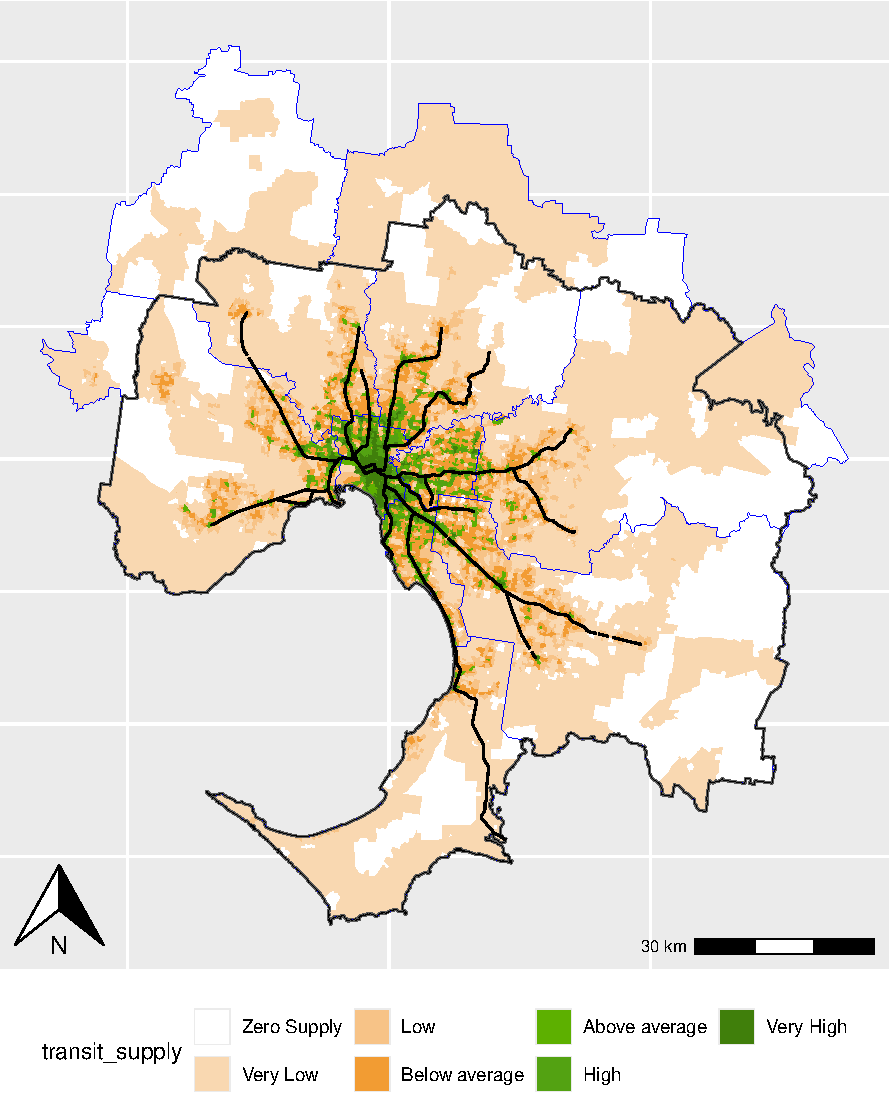
\includegraphics{Leveraging_GTFS_to_assess_transit_supply_Transport_Geography_files/figure-latex/Greater_Melbourne_2021_SA1_plot-1.pdf}
\caption{Greater Melbourne, Transit Supply by SA1 for the week starting
the date of the 2021 census, overlayed with: 2006 Greater Melbourne
boundary (black); 2021 SA4 boundaries (blue); and suburban railway lines
(black)}
\end{figure}

\begin{table}

\caption{\label{tab:Greater_Melbourne_CCDs_SA1_table}Distribution of 2006, 2016 and 2021 Transport Supply to Melbourne CCDs (2006 boundaries), 2016 Transport Supply to Greater Melbourne (2016 SA1s) and 2021 Transport Supply to Greater Melbourne (2021 SA1s). Sources: 2006 values, Currie (2010); 2016 and 2021 values, authors' analysis}
\centering
\begin{tabular}[t]{l|r|r|r|r|r}
\hline
\multicolumn{1}{c|}{Transport} & \multicolumn{3}{c|}{CCDs} & \multicolumn{1}{c|}{2016 SA1s} & \multicolumn{1}{c}{2021 SA1s} \\
\cline{1-1} \cline{2-4} \cline{5-5} \cline{6-6}
Supply & 2006 & 2016 & 2021 & 2016 & 2021\\
\hline
Zero Supply & 3.2\%   (189) & 1.4\%    (86) & 1.3\%    (81) & 3.2\%    (326) & 4.3\%    (489)\\
\hline
Very Low & 22.5\% (1,314) & 23.5\% (1,485) & 23.3\% (1,474) & 23.0\%  (2,362) & 23.4\%  (2,692)\\
\hline
Low & 22.4\% (1,310) & 23.5\% (1,484) & 23.3\% (1,473) & 23.0\%  (2,362) & 23.4\%  (2,691)\\
\hline
Below average & 22.2\% (1,294) & 23.5\% (1,484) & 23.3\% (1,473) & 23.0\%  (2,362) & 23.4\%  (2,691)\\
\hline
Above average & 10.4\%   (608) & 9.4\%   (596) & 9.6\%   (608) & 9.3\%    (959) & 8.5\%    (975)\\
\hline
High & 9.2\%   (535) & 9.4\%   (595) & 9.6\%   (608) & 9.3\%    (959) & 8.5\%    (974)\\
\hline
Very High & 10.1\%   (589) & 9.4\%   (595) & 9.6\%   (608) & 9.3\%    (959) & 8.5\%    (975)\\
\hline
Total & 100.0\% (5,839) & 100.0\% (6,325) & 100.0\% (6,325) & 100.0\% (10,289) & 100.0\% (11,487)\\
\hline
\end{tabular}
\end{table}

Table \ref{tab:Greater_Melbourne_CCDs_SA1_table} summarises the
distribution of CCDs and SA1s across different Transport Supply
categories in 2006, 2016 and 2021. Figure
\ref{fig:Greater_Melbourne_2021_SA1_plot} shows the spatial distribution
of Transport Supply in 2021. Maps for 2016 and CCDs are included in the
Appendix.

There is a statistically significant difference in the shares of CCDs in
each category between 2006, 2016 and 2021
(\(\chi^2(12, N = 18489) = 87.45\), \(p < .001\)). Only 81 CCDs (1.3\%)
have Zero Supply in 2021, compared to the 189 (3.2\%) reported by
\citet{currie2010identifying} for 2006. Differences are also
statistically significant when comparing 2006 and 2016
(\(\chi^2(6, N = 12164) = 56.87\), \(p < .001\)) or 2006 and 2021
\(\chi^2(6, N = 12164) = 59.15\), \(p < .001\)), but not between 2016
and 2021 (\(\chi^2(6, N = 12650) = 0.67\), \(p = .995\)).

These values, however, are only for CCDs within the 2006 extents of
Melbourne. The ABS' statistical boundary of ``Greater Melbourne'' now
includes areas up to around 30 kilometers further to the north, as shown
in the 2021 map in Figure \ref{fig:Greater_Melbourne_2021_SA1_plot}.
This shows that the new parts of Melbourne, beyond the 2006 statistical
boundary, mostly have Very Low or Zero Transport Supply levels. Again,
the differences between 2006 (CCDs), 2016 and 2021 (SA1s) are
statistically significant (\(\chi^2(12, N = 27615) = 58.86\),
\(p < .001\)), but not between 2006 and 2016 (as a pair,
\(\chi^2(6, N = 16128) = 8.83\), \(p = .183\)). The differences between
2006 and 2021 are statistically significant
(\(\chi^2(6, N = 17326) = 44.83\), \(p < .001\)) as are the differences
between 2016 and 2021 \(\chi^2(6, N = 21776) = 31.56\), \(p < .001\)).
There are a greater proportion of SA1s with Zero Supply in 2021 (4.3\%)
than there were CCDs in 2006 (3.25\%) or SA1s in 2016 (3.2\%) . The
share of SA1s with supply below the average SI score (i.e.~Zero, Very
Low, Low or Below Average) is also larger in 2021 (74.5\%) compared to
the share of CCDs in 2006 (70.3\%) or share of SA1s in 2016 (72.0\%)

\begin{table}

\caption{\label{tab:Greater_Melbourne_CCDs_SA1_population}Distribution of 2006, 2016 and 2021 Transport Supply to population in Melbourne. Sources: 2006 values, Currie (2010); 2016 and 2021 values, authors' analysis}
\centering
\begin{tabular}[t]{l|r|r|r}
\hline
Supply & 2006 & 2016 & 2021\\
\hline
Zero Supply & 2.5\%    (85,423) & 2.9\%   (131,619) & 3.8\%   (186,829)\\
\hline
Very Low & 23.6\%   (793,046) & 22.5\% (1,008,498) & 23.0\% (1,132,967)\\
\hline
Low & 25.7\%   (865,330) & 22.7\% (1,016,848) & 23.7\% (1,163,358)\\
\hline
Below average & 23.0\%   (774,521) & 22.3\% (1,000,290) & 23.6\% (1,159,783)\\
\hline
Above average & 9.6\%   (324,546) & 9.3\%   (418,614) & 8.7\%   (426,892)\\
\hline
High & 7.7\%   (260,411) & 9.6\%   (428,880) & 8.7\%   (425,779)\\
\hline
Very High & 7.8\%   (263,832) & 10.7\%   (480,469) & 8.6\%   (422,025)\\
\hline
Total & 100.0\% (3,367,109) & 100.0\% (4,485,218) & 100.0\% (4,917,633)\\
\hline
\end{tabular}
\end{table}

Table \ref{tab:Greater_Melbourne_CCDs_SA1_population} compares the share
of resident population in each transport supply category. Differences
are statistically significant across all three (2006, 2016 and 2021
\(\chi^2(12, N = 12769960) = 51092.54\), \(p < .001\)), between 2006 and
2016 (\(\chi^2(6, N = 7852327) = 34135.14\), \(p < .001\)), and between
2006 and 2021 (\(\chi^2(6, N = 8284742) = 19038.97\), \(p < .001\)). The
number of people with zero supply rose from 85,423 (2.5\%) in 2006 to
186,829 (3.8\%) in 2021. This represents a 118.7\% increase, compared to
the population increase of 46.0\% across all of Greater Melbourne. The
number of people with zero or very low supply rose from 878,469 (26.1\%)
in 2006 to 1,319,796 (26.8\%) in 2021. This represents a 50.2\% increase
(4.2\% higher than the population change). The number of people with a
supply that was below the average (Zero, Very Low, Low or Below Average)
rose from 2,518,320 (74.8\%) in 2006 to 3,642,937 (74.1\%) in 2021. This
represents a 44.7\% increase (1.4\% lower than the population change).

Differences were also statistically significant between 2016 and 2021
(\(\chi^2(6, N = 9402851) = 22467.17\), \(p < .001\)). The number of
people with zero supply rose from 131,619 (2.9\%) in 2016 by 55,210
people (a 41.9\% increase), compared to the overall population increase
of 9.6\% in Greater Melbourne between 2016 and 2021. The number of
people with zero or very low supply rose from 1,140,117 (25.4\% of the
population) by 179,679 (a 15.8\% increase), while the number with a
supply that was below the average (Zero, Very Low, Low or Below Average)
rose from 3,157,255 (70.4\% of the population) by 485,682 people (an
increase of 15.4\%).

\begin{table}

\caption{\label{tab:Greater_Melbourne_population_2016_by_SA4}Greater Melbourne 2016: Share of population in each Transport Supply category for each SA4 region}
\centering
\fontsize{8}{10}\selectfont
\begin{tabular}[t]{>{\raggedright\arraybackslash}p{1.75cm}|>{\raggedleft\arraybackslash}p{1cm}|>{\raggedleft\arraybackslash}p{1cm}|>{\raggedleft\arraybackslash}p{1cm}|>{\raggedleft\arraybackslash}p{1cm}|>{\raggedleft\arraybackslash}p{1cm}|>{\raggedleft\arraybackslash}p{1cm}|>{\raggedleft\arraybackslash}p{1cm}|>{\raggedright\arraybackslash}p{1cm}|>{\raggedleft\arraybackslash}p{1cm}|>{\raggedleft\arraybackslash}p{1.25cm}}
\hline
Transport Supply & Inner & Inner East & Inner South & North East & North West & Outer East & South East & West & M'ton Pen. & Total\\
\hline
Zero Supply & 0.0\%       (0) & 0.0\%     (480) & 0.0\%   (1,604) & 0.4\%  (16,988) & 0.4\%  (17,655) & 0.3\%  (12,955) & 1.0\%  (44,757) & 0.3\%  (12,056) & 0.6\%  (25,124) & 2.9\%   (131,619)\\
\hline
Very Low & 0.1\%   (3,427) & 0.4\%  (18,454) & 0.6\%  (24,944) & 2.5\% (112,269) & 2.1\%  (94,853) & 4.3\% (190,890) & 4.8\% (215,217) & 4.2\% (186,665) & 3.6\% (161,779) & 22.5\% (1,008,498)\\
\hline
Low & 0.4\%  (18,018) & 0.9\%  (39,235) & 1.4\%  (60,833) & 2.7\% (119,608) & 2.4\% (107,693) & 3.0\% (135,247) & 5.0\% (224,097) & 5.4\% (242,438) & 1.6\%  (69,679) & 22.7\% (1,016,848)\\
\hline
Below average & 1.0\%  (42,950) & 2.3\% (105,168) & 2.9\% (128,014) & 2.9\% (132,008) & 2.2\%  (97,739) & 2.7\% (119,691) & 4.0\% (177,817) & 3.8\% (170,015) & 0.6\%  (26,888) & 22.3\% (1,000,290)\\
\hline
Above average & 1.0\%  (44,547) & 1.8\%  (80,002) & 1.8\%  (81,038) & 1.0\%  (46,965) & 0.6\%  (28,905) & 0.6\%  (25,188) & 1.2\%  (53,228) & 1.2\%  (54,895) & 0.1\%   (3,846) & 9.3\%   (418,614)\\
\hline
High & 2.9\% (129,533) & 1.7\%  (74,966) & 1.7\%  (74,617) & 1.0\%  (46,291) & 0.3\%  (14,464) & 0.3\%  (15,371) & 0.7\%  (33,365) & 0.9\%  (38,499) & 0.0\%   (1,774) & 9.6\%   (428,880)\\
\hline
Very High & 7.9\% (353,232) & 0.9\%  (41,416) & 0.7\%  (32,561) & 0.5\%  (21,197) & 0.0\%   (2,033) & 0.0\%     (314) & 0.2\%   (6,893) & 0.5\%  (22,823) & 0.0\%       (0) & 10.7\%   (480,469)\\
\hline
Total & 13.2\% (591,707) & 8.0\% (359,721) & 9.0\% (403,611) & 11.0\% (495,326) & 8.1\% (363,342) & 11.1\% (499,656) & 16.8\% (755,374) & 16.2\% (727,391) & 6.4\% (289,090) & 100.0\% (4,485,218)\\
\hline
\end{tabular}
\end{table}

\begin{table}

\caption{\label{tab:Greater_Melbourne_population_2021_by_SA4}Greater Melbourne 2021: Share of population in each Transport Supply category for each SA4 region}
\centering
\fontsize{8}{10}\selectfont
\begin{tabular}[t]{>{\raggedright\arraybackslash}p{1.75cm}|>{\raggedleft\arraybackslash}p{1cm}|>{\raggedleft\arraybackslash}p{1cm}|>{\raggedleft\arraybackslash}p{1cm}|>{\raggedleft\arraybackslash}p{1cm}|>{\raggedleft\arraybackslash}p{1cm}|>{\raggedleft\arraybackslash}p{1cm}|>{\raggedleft\arraybackslash}p{1cm}|>{\raggedright\arraybackslash}p{1cm}|>{\raggedleft\arraybackslash}p{1cm}|>{\raggedleft\arraybackslash}p{1.25cm}}
\hline
Transport Supply & Inner & Inner East & Inner South & North East & North West & Outer East & South East & West & M'ton Pen. & Total\\
\hline
Zero Supply & 0.0\%       (0) & 0.3\%     (478) & 0.9\%   (1,655) & 14.2\%  (26,563) & 11.9\%  (22,186) & 7.6\%  (14,125) & 28.9\%  (53,966) & 23.5\%  (43,898) & 12.8\%  (23,958) & 100.0\%   (186,829)\\
\hline
Very Low & 0.4\%   (4,169) & 1.8\%  (20,688) & 2.0\%  (22,483) & 11.5\% (130,715) & 9.8\% (110,814) & 17.7\% (200,810) & 22.1\% (250,684) & 19.5\% (221,337) & 15.1\% (171,267) & 100.0\% (1,132,967)\\
\hline
Low & 1.7\%  (20,329) & 3.9\%  (45,160) & 5.5\%  (63,802) & 11.3\% (132,001) & 10.6\% (123,314) & 13.4\% (155,603) & 22.9\% (265,995) & 24.9\% (289,518) & 5.8\%  (67,636) & 100.0\% (1,163,358)\\
\hline
Below average & 4.7\%  (54,918) & 11.5\% (133,305) & 12.8\% (148,585) & 13.0\% (151,240) & 11.2\% (129,918) & 9.9\% (114,658) & 17.6\% (204,093) & 15.9\% (184,466) & 3.3\%  (38,600) & 100.0\% (1,159,783)\\
\hline
Above average & 13.2\%  (56,422) & 16.2\%  (69,199) & 21.8\%  (92,875) & 10.4\%  (44,470) & 6.4\%  (27,140) & 5.2\%  (22,262) & 12.5\%  (53,328) & 13.0\%  (55,438) & 1.3\%   (5,758) & 100.0\%   (426,892)\\
\hline
High & 35.6\% (151,439) & 17.3\%  (73,687) & 16.3\%  (69,281) & 10.3\%  (43,985) & 2.3\%   (9,710) & 2.6\%  (10,905) & 5.8\%  (24,707) & 9.7\%  (41,100) & 0.2\%     (965) & 100.0\%   (425,779)\\
\hline
Very High & 78.1\% (329,654) & 7.3\%  (30,949) & 5.7\%  (23,906) & 2.8\%  (11,752) & 0.3\%   (1,285) & 0.0\%       (0) & 1.7\%   (7,308) & 4.1\%  (17,171) & 0.0\%       (0) & 100.0\%   (422,025)\\
\hline
Total & 12.5\% (616,931) & 7.6\% (373,466) & 8.6\% (422,587) & 11.0\% (540,726) & 8.6\% (424,367) & 10.5\% (518,363) & 17.5\% (860,081) & 17.3\% (852,928) & 6.3\% (308,184) & 100.0\% (4,917,633)\\
\hline
\end{tabular}
\end{table}

Table \ref{tab:Greater_Melbourne_population_2016_by_SA4} and Table
\ref{tab:Greater_Melbourne_population_2021_by_SA4} show the distribution
of Transport Supply categories to the population in each SA4 zone in
2016 and 2021 respectively\footnote{SA4s are the largest of the
  statistical boundaries used by the ABS for areas smaller than Greater
  Capital Cities or other agglomerations.}. Variations across SA4 zones
are statistically significant in both 2016
(\(\chi^2(48, N = 4485218) = 2847273.25\), \(p < .001\)) and 2021
(\(\chi^2(48, N = 4917633) = 3126013.64\), \(p < .001\)). In general,
outer areas of Greater Melbourne\footnote{The North East, North West,
  Outer East, South East, West and Mornington Peninsula SA4 zones}
appear to have larger shares of residents living in areas with Transport
Supply that is lower than the average. In 2016 2,714,128 residents
(60.5\% of the total population of Greater Melbourne) were both living
outside of the inner three SA4s and in SA1s with lower than average
transport supply. By 2021 this had increased to 3,127,365 residents
(63.6\% of the total population).

\subsubsection{Supply Index scores}\label{supply-index-scores}

\citet{currie2010identifying} reported an average SI score for CCDs in
2006 of 2,886.9 across Melbourne. The average SI value in 2021 (using
CCDs and within the 2006 boundary) was 3,390. SI scores average
12,275.7, 3,409.1 and 998.96 in 2021 for the CCDs in the inner, middle
and outer suburbs respectively\footnote{The same grouping of LGAs to
  inner, middle and outer suburb groups as used in
  \citet{currie2010identifying} was used for this analysis, although
  here the City of Stonnington was allocated entirely to the middle
  grouping, whereas \citet{currie2010identifying} allocated part of this
  LGA to the inner group.}, compared to 10,922.7, 2,694.9 and 764.3,
respectively, reported for 2006 in \citet{currie2010identifying}.
However, the \citet{currie2010identifying} show 5,839 total CCDs within
Melbourne, whereas the shape files obtained for this analysis include
6,325 CCDs within the 2006 Melbourne boundary. Hence, results found here
might not be exactly comparable to those in
\citet{currie2010identifying} due to geographic inconsistencies,
although overall results appear to be consistent with there having been
increases in SI scores across all parts of Melbourne since 2006 and the
general pattern of higher average SI scores in inner and then middle
suburbs remaining unchanged.

\begin{table}

\caption{\label{tab:Greater_Melbourne_2016_2021_ratio_map}Greater Melbourne: Share of 2021 population living in SA1s by change in transit service (2016 vs 2021) by SA4 region}
\centering
\fontsize{8}{10}\selectfont
\begin{tabular}[t]{>{\raggedright\arraybackslash}p{1.75cm}|>{\raggedleft\arraybackslash}p{1cm}|>{\raggedleft\arraybackslash}p{1cm}|>{\raggedleft\arraybackslash}p{1cm}|>{\raggedleft\arraybackslash}p{1cm}|>{\raggedleft\arraybackslash}p{1cm}|>{\raggedleft\arraybackslash}p{1cm}|>{\raggedleft\arraybackslash}p{1cm}|>{\raggedright\arraybackslash}p{1cm}|>{\raggedleft\arraybackslash}p{1cm}|>{\raggedleft\arraybackslash}p{1.25cm}}
\hline
Change & Inner & Inner East & Inner South & North East & North West & Outer East & South East & West & M'ton Pen. & Total\\
\hline
Never served & 0.0\%       (0) & 0.0\%     (478) & 0.0\%   (1,655) & 0.5\%  (24,786) & 0.4\%  (21,762) & 0.3\%  (12,855) & 1.1\%  (52,606) & 0.9\%  (42,883) & 0.5\%  (23,958) & 3.7\%   (180,983)\\
\hline
New service & 0.0\%       (0) & 0.0\%       (0) & 0.0\%       (0) & 0.2\%   (9,911) & 0.7\%  (36,817) & 0.0\%     (238) & 1.1\%  (53,254) & 0.8\%  (40,483) & 0.1\%   (3,038) & 2.9\%   (143,741)\\
\hline
Increased 30\% or more & 0.0\%   (1,843) & 0.0\%     (279) & 0.8\%  (37,932) & 0.9\%  (46,448) & 1.7\%  (83,007) & 0.1\%   (4,209) & 2.6\% (127,248) & 2.7\% (131,194) & 1.3\%  (65,724) & 10.1\%   (497,884)\\
\hline
Increased 10 to 30\% & 0.9\%  (45,197) & 0.1\%   (3,190) & 0.8\%  (41,577) & 0.8\%  (40,989) & 1.1\%  (56,013) & 0.5\%  (22,609) & 1.6\%  (77,391) & 2.1\% (101,767) & 0.4\%  (21,060) & 8.3\%   (409,793)\\
\hline
Increased 5 to 10\% & 1.5\%  (72,360) & 0.3\%  (13,018) & 1.1\%  (52,033) & 0.8\%  (37,258) & 0.6\%  (31,400) & 0.5\%  (26,666) & 1.1\%  (53,370) & 2.1\% (101,769) & 0.2\%  (10,149) & 8.1\%   (398,023)\\
\hline
Increased 3 to 5\% & 1.6\%  (79,047) & 0.5\%  (25,074) & 0.6\%  (30,595) & 1.2\%  (60,661) & 1.1\%  (55,445) & 0.5\%  (23,819) & 0.9\%  (45,773) & 1.8\%  (88,601) & 0.3\%  (14,666) & 8.6\%   (423,681)\\
\hline
Increased 1 to 3\% & 2.3\% (115,203) & 1.4\%  (67,357) & 1.2\%  (60,889) & 1.9\%  (92,896) & 0.9\%  (42,761) & 0.8\%  (39,263) & 1.5\%  (75,676) & 2.4\% (117,967) & 0.7\%  (32,811) & 13.1\%   (644,823)\\
\hline
Within 1\% & 2.6\% (128,666) & 3.8\% (187,974) & 2.0\%  (97,037) & 2.5\% (124,942) & 1.2\%  (57,899) & 5.6\% (274,423) & 5.4\% (266,787) & 3.0\% (146,702) & 2.2\% (109,151) & 28.3\% (1,393,581)\\
\hline
Reduced 1 to 3\% & 1.0\%  (49,729) & 0.8\%  (39,675) & 0.6\%  (27,179) & 0.7\%  (34,180) & 0.3\%  (13,986) & 0.8\%  (38,826) & 0.7\%  (34,125) & 0.4\%  (19,517) & 0.4\%  (18,446) & 5.6\%   (275,663)\\
\hline
Reduced 3 to 10\% & 1.8\%  (89,662) & 0.5\%  (25,930) & 0.9\%  (42,701) & 0.9\%  (44,261) & 0.2\%  (11,175) & 0.9\%  (43,143) & 0.5\%  (24,903) & 0.7\%  (33,329) & 0.2\%   (7,953) & 6.6\%   (323,057)\\
\hline
Reduced by more than 10\% & 0.7\%  (35,224) & 0.2\%  (10,491) & 0.6\%  (30,989) & 0.5\%  (22,617) & 0.3\%  (13,678) & 0.6\%  (31,042) & 1.0\%  (47,588) & 0.6\%  (27,701) & 0.0\%   (1,228) & 4.5\%   (220,558)\\
\hline
Service withdrawn & 0.0\%       (0) & 0.0\%       (0) & 0.0\%       (0) & 0.0\%   (1,777) & 0.0\%     (424) & 0.0\%   (1,270) & 0.0\%   (1,360) & 0.0\%   (1,015) & 0.0\%       (0) & 0.1\%     (5,846)\\
\hline
Total & 12.5\% (616,931) & 7.6\% (373,466) & 8.6\% (422,587) & 11.0\% (540,726) & 8.6\% (424,367) & 10.5\% (518,363) & 17.5\% (860,081) & 17.3\% (852,928) & 6.3\% (308,184) & 100.0\% (4,917,633)\\
\hline
\end{tabular}
\end{table}

\begin{figure}
\centering
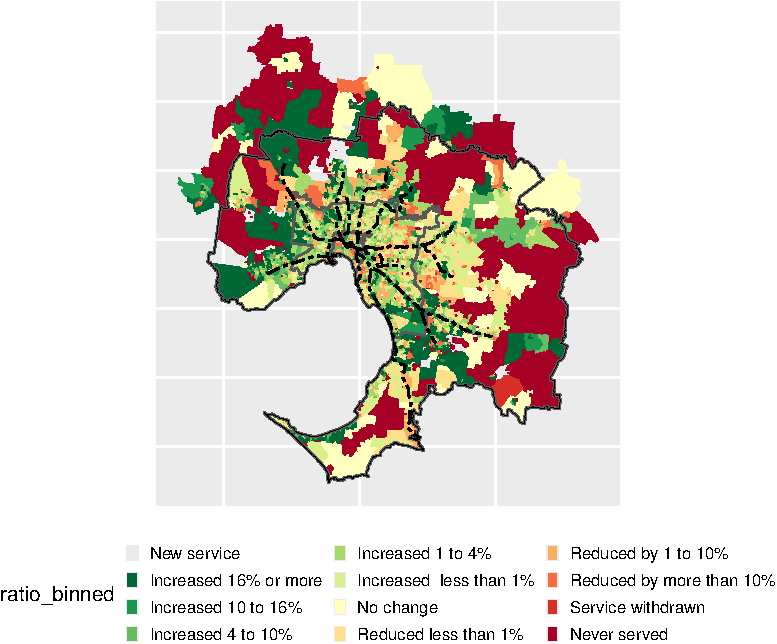
\includegraphics{Leveraging_GTFS_to_assess_transit_supply_Transport_Geography_files/figure-latex/Greater_Melbourne_2016_2021_ratio_map-1.pdf}
\caption{Greater Melbourne: changes in SI between 2016 and 2021, by 2021
SA1, overlayed with SA4 boundaries (blue) and suburban railway lines
(black)}
\end{figure}

It is, however, possible to directly compare SI scores 2016 and 2021.
Average SI scores for all of Greater Melbourne (SA1 2021 boundaries)
increased from 2,843.8 in 2016 to 2,901.4 in 2021 (+2.0\%). There is a
statistically significant and strong correlation between the 2016 and
2021 SI scores (\(r(11485) = 1.00\), \(p < .001\), \(r_s =.98\),
\(p < .001\)).

Table \ref{tab:Greater_Melbourne_2016_2021_ratio_map} shows changes in
SI score between 2016 and 2021 (column 1) by 2021 SA1s for the 2021
population, summarised for each SA4 zone (columns 2 to 10) and Greater
Melbourne as a whole (column 11). These are mapped in Figure
\ref{fig:Greater_Melbourne_2016_2021_ratio_map}.There is a statistically
significant difference in the distribution of service level changes
across the populations between SA4 areas
(\(\chi^2(88, N = 4917633) = 1220826.77\), \(p < .001\)). In 2021, more
than half of the population were living in SA1s where the SI scores were
more than one percent higher than in 2016 in the North-West (305,443
people, 72.0\%), West (581,781 people, 68.2\%), North East (288,163
people, 53.3\%), South East (432,712 people, 50.7\%), Mornington
Peninsula (147,448 people, 47.8\%) and Inner (313,650 people, 50.8\%)
SA4s

Service levels in 2021 were within one percent of the level in 2016 for
most of the population in the Outer East (52.9\%) and Inner East
(50.3\%), compared to only 28.3\% of the population across all of
Greater Melbourne. The largest shares of the population living in areas
were service levels remained within one percent were in the Outer East
(274,423 people, 19.7\% of the 1,393,581), South East (266,787 people,
19.1\%) and Inner East (187,974 people, 13.5\%).

In 2021, the share of the population living in SA1s where the SI was one
or more percent lower than in 2016 was largest in the Inner (28.3\%),
Inner South (23.9\%) and Outer East (22.0\%) SA4s. The largest shares of
residents with at less one percent lower service level in 2021 were
among the Inner (174,615), Outer East (114,281) and South East (107,976)
SA4 areas.

\subsubsection{Social needs}\label{social-needs}

\begin{figure}
\centering
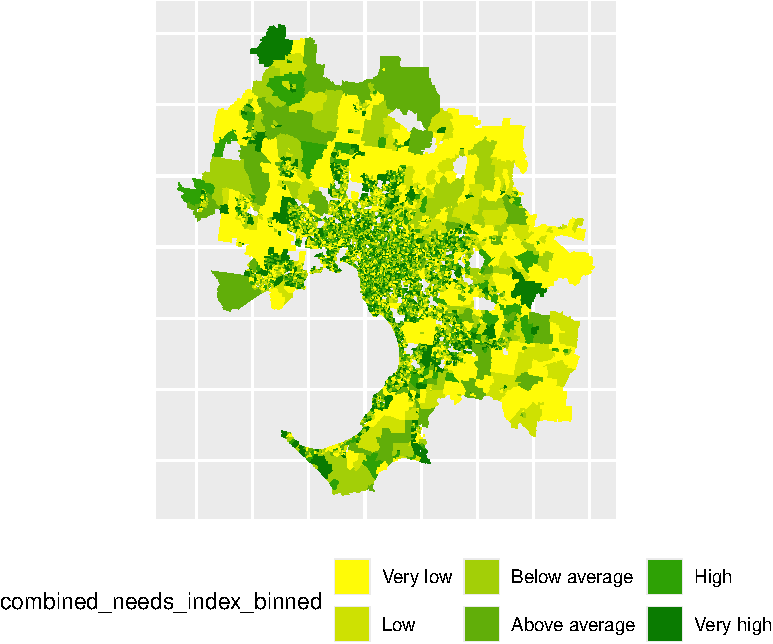
\includegraphics{Leveraging_GTFS_to_assess_transit_supply_Transport_Geography_files/figure-latex/Greater_Melbourne_2021_social_needs-1.pdf}
\caption{Distribution of categories of composite social need index
scores, overlayed with: 2006 Greater Melbourne boundary (black); SA4
boundaries (blue); and suburban railway lines (dashed).}
\end{figure}

Figure \ref{fig:Greater_Melbourne_2021_social_needs} shows the
distribution of categories of social need index scores across Greater
Melbourne for 2021\footnote{A map for 2016 is included in the Appendix
  as Figure
  \textbackslash ref\{fig:Greater\_Melbourne\_2016\_social\_needs\_appendix}.
This is analogous to the 2006 map shown in Figure
\ref{fig:Currie_map_SI} (middle) although, as discussed in the
methodology section above, it was not possible to exactly replicate the
\citet{currie2010identifying} social needs scoring approach due to
changes in the way census results are reported. In general, the spatial
grouping of different levels of social need appears less consistently
grouped in 2021 than in 2006, although this may be an artifact of the
shift to SA1s from CCDs\footnote{CCDs were originally devised to group
  the approximately 200 dwellings allocated to each individual census
  collector, whereas SA1s were introduced to be consistent in population
  (200 to 800 people, averaging 400) and character \citep{ABS_SA1s_CCDs}}.

\subsubsection{Needs-gap}\label{needs-gap}

\begin{figure}
\centering
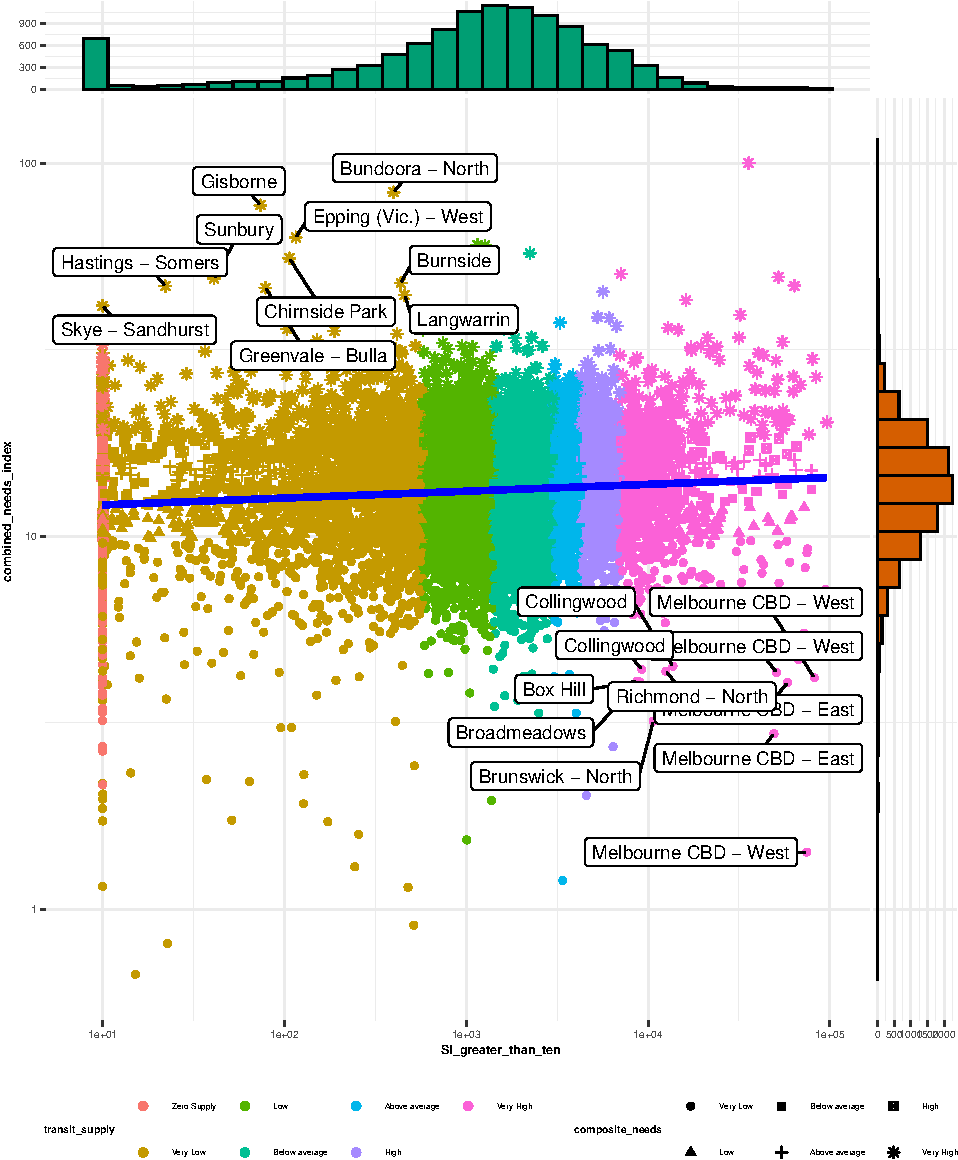
\includegraphics{Leveraging_GTFS_to_assess_transit_supply_Transport_Geography_files/figure-latex/Greater_Melbourne_2021_needs_gap_scatterplot_figure-1.pdf}
\caption{Greater Melbourne 2021, SI and Combined Needs Index scores,
with SI scores \textless{} 10 rounded up to equal 10.}
\end{figure}

Figures \ref{fig:Greater_Melbourne_2016_needs_gap_scatterplot_figure}
and \ref{fig:Greater_Melbourne_2016_needs_gap_scatterplot_figure} show
social needs and SI scores\footnote{To improve the clarity of the
  figure, SI scores less than 10 have been adjusted to equal 10.}. Those
SA1s with combinations of Zero or Very Low transit supply and
(especially) high needs scores (more than 40); or Very High supply and
Very Low needs scores (less than 4.5) have been labels with their SA2
name, so as to given an indication of which suburbs of Melbourne are at
each of the extremes. There is a significant, but only weakly positive
correlation between the SI and Combined Needs Index scores for both 2016
(\(r(11136) = .06\), \(p < .001\), \(r_s =.07\), \(p < .001\)) and 2021
(\(r(11136) = .06\), \(p < .001\), \(r_s =.07\), \(p < .001\)).

Table \ref{tab:Greater_Melbourne_2016_needs_gap_population} compares the
populations within each Transport Supply and Combined Needs Index
grouping for 2016. There is a statistically significant relationship
(\(\chi^2(30, N = 4471171) = 158778.27\), \(p < .001\)). 301,743 people
live within SA1s that have Zero or Very Low transport supply, but Very
High social needs. This represents 6.7\% of the 4,471,171 people within
Greater Melbourne, and is higher proportion than that reported for 2006
(139,004 of 3.3 million people (4.2\%)).

Table \ref{tab:Greater_Melbourne_2021_needs_gap_population} shows the
same comparison for 2021. There is a statistically significant
relationship (\(\chi^2(30, N = 4904313) = 55715.62\), \(p < .001\)).
333,887 people live within SA1s that have Zero or Very Low transport
supply, but Very High social needs. This represents 6.8\% of the
4,904,313 people within Greater Melbourne, which is higher than that
reported for both 2006 and 2016.

\begin{table}

\caption{\label{tab:Greater_Melbourne_2016_needs_gap_population}Greater Melbourne 2016, Population in each SI and Combined Needs Index grouping}
\centering
\fontsize{8}{10}\selectfont
\begin{tabular}[t]{>{\raggedright\arraybackslash}p{2.5cm}|>{\raggedleft\arraybackslash}p{1cm}|>{\raggedleft\arraybackslash}p{1cm}|>{\raggedleft\arraybackslash}p{1cm}|>{\raggedright\arraybackslash}p{1cm}|>{\raggedleft\arraybackslash}p{1cm}|>{\raggedleft\arraybackslash}p{1cm}|>{\raggedleft\arraybackslash}p{1.5cm}}
\hline
\multicolumn{1}{c|}{ } & \multicolumn{6}{c|}{Combined Needs Index Category} & \multicolumn{1}{c}{ } \\
\cline{2-7}
Supply & Very High & High & Above Average & Below Average & Low & Very Low & Total\\
\hline
Zero Supply & 0.9\%    (38,050) & 0.3\%  (14,790) & 0.3\%  (15,402) & 0.4\%  (18,784) & 0.5\%  (22,544) & 0.5\%  (22,012) & 2.9\%   (131,582)\\
\hline
Very Low & 5.9\%   (263,693) & 3.4\% (153,169) & 3.1\% (138,710) & 3.7\% (165,350) & 3.5\% (156,359) & 2.8\% (126,298) & 22.4\% (1,003,579)\\
\hline
Low & 4.5\%   (200,937) & 3.8\% (168,541) & 3.5\% (154,275) & 4.4\% (197,542) & 3.8\% (168,228) & 2.8\% (126,411) & 22.7\% (1,015,934)\\
\hline
Below average & 3.7\%   (164,681) & 4.0\% (177,044) & 3.7\% (163,593) & 4.3\% (193,915) & 3.8\% (169,849) & 2.9\% (129,440) & 22.3\%   (998,522)\\
\hline
Above average & 1.9\%    (84,562) & 1.8\%  (80,172) & 1.6\%  (70,066) & 1.8\%  (80,591) & 1.4\%  (61,679) & 0.8\%  (38,003) & 9.3\%   (415,073)\\
\hline
High & 2.4\%   (105,960) & 2.0\%  (89,517) & 1.5\%  (67,061) & 1.9\%  (83,055) & 1.1\%  (49,615) & 0.7\%  (33,334) & 9.6\%   (428,542)\\
\hline
Very High & 4.3\%   (192,038) & 1.8\%  (79,329) & 1.5\%  (68,467) & 1.3\%  (56,303) & 1.1\%  (48,441) & 0.7\%  (33,361) & 10.7\%   (477,939)\\
\hline
Total & 23.5\% (1,049,921) & 17.1\% (762,562) & 15.2\% (677,574) & 17.8\% (795,540) & 15.1\% (676,715) & 11.4\% (508,859) & 100.0\% (4,471,171)\\
\hline
\end{tabular}
\end{table}

\begin{table}

\caption{\label{tab:Greater_Melbourne_2021_needs_gap_population}Greater Melbourne 2021, Population in each SI and Combined Needs Index grouping}
\centering
\fontsize{8}{10}\selectfont
\begin{tabular}[t]{>{\raggedright\arraybackslash}p{2.5cm}|>{\raggedleft\arraybackslash}p{1cm}|>{\raggedleft\arraybackslash}p{1cm}|>{\raggedleft\arraybackslash}p{1cm}|>{\raggedright\arraybackslash}p{1cm}|>{\raggedleft\arraybackslash}p{1cm}|>{\raggedleft\arraybackslash}p{1cm}|>{\raggedleft\arraybackslash}p{1.5cm}}
\hline
\multicolumn{1}{c|}{ } & \multicolumn{6}{c|}{Combined Needs Index Category} & \multicolumn{1}{c}{ } \\
\cline{2-7}
Supply & Very High & High & Above Average & Below Average & Low & Very Low & Total\\
\hline
Zero Supply & 0.9\%    (41,915) & 0.6\%  (27,179) & 0.5\%  (22,705) & 0.7\%  (32,328) & 0.7\%  (32,645) & 0.6\%  (30,002) & 3.8\%   (186,774)\\
\hline
Very Low & 6.0\%   (291,972) & 4.1\% (199,467) & 3.4\% (165,968) & 3.7\% (182,624) & 3.2\% (158,222) & 2.6\% (129,608) & 23.0\% (1,127,861)\\
\hline
Low & 4.9\%   (239,199) & 4.2\% (205,465) & 3.9\% (193,243) & 4.3\% (210,576) & 3.7\% (183,333) & 2.7\% (130,779) & 23.7\% (1,162,595)\\
\hline
Below average & 4.7\%   (228,646) & 4.5\% (219,310) & 4.2\% (204,049) & 4.2\% (203,750) & 3.5\% (171,997) & 2.7\% (130,322) & 23.6\% (1,158,074)\\
\hline
Above average & 2.0\%   (100,326) & 1.6\%  (80,404) & 1.5\%  (73,669) & 1.6\%  (76,179) & 1.2\%  (56,902) & 0.8\%  (37,419) & 8.7\%   (424,899)\\
\hline
High & 2.2\%   (107,121) & 1.7\%  (83,970) & 1.4\%  (70,132) & 1.6\%  (77,358) & 1.1\%  (54,528) & 0.7\%  (32,274) & 8.7\%   (425,383)\\
\hline
Very High & 2.6\%   (129,759) & 1.6\%  (79,306) & 1.2\%  (59,356) & 1.1\%  (55,828) & 1.1\%  (54,061) & 0.8\%  (40,417) & 8.5\%   (418,727)\\
\hline
Total & 23.2\% (1,138,938) & 18.3\% (895,101) & 16.1\% (789,122) & 17.1\% (838,643) & 14.5\% (711,688) & 10.8\% (530,821) & 100.0\% (4,904,313)\\
\hline
\end{tabular}
\end{table}

\begin{figure}
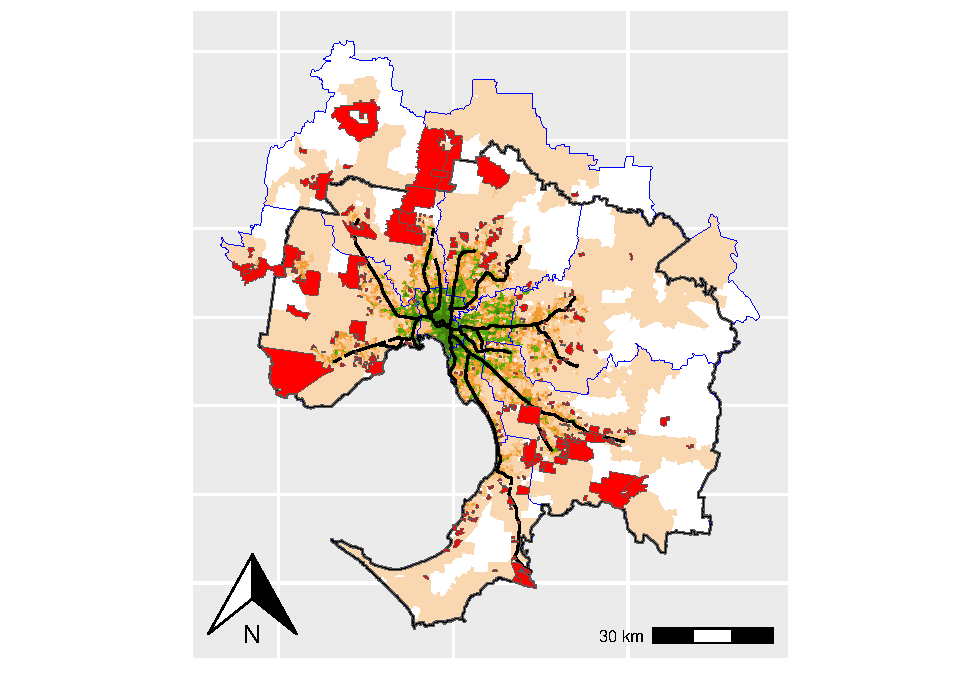
\includegraphics[width=1\linewidth]{Leveraging_GTFS_to_assess_transit_supply_Transport_Geography_files/figure-latex/Greater_Melbourne_2016_needs_gap_map_figure-1} \caption{Greater Melbourne 2016 SI groupings, overlayed with SA1s with very high transport need areas with zero or very low public transport supply (red).}\label{fig:Greater_Melbourne_2016_needs_gap_map_figure}
\end{figure}

\begin{figure}
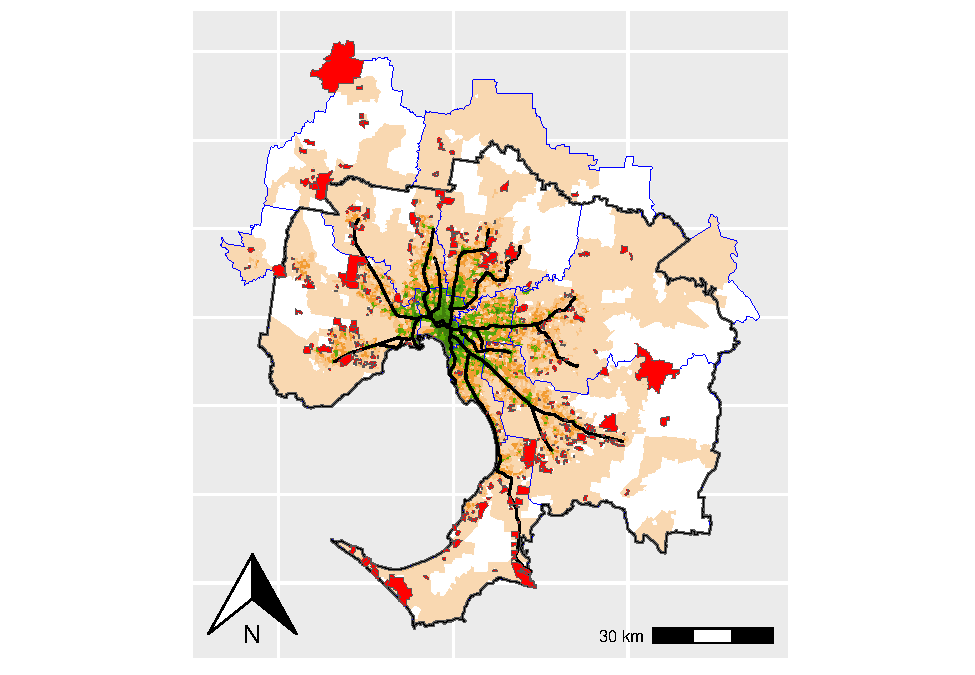
\includegraphics[width=1\linewidth]{Leveraging_GTFS_to_assess_transit_supply_Transport_Geography_files/figure-latex/Greater_Melbourne_2021_needs_gap_map_figure-1} \caption{Greater Melbourne 2021 SI groupings, overlayed with SA1s with very high transport need areas with zero or very low public transport supply (red).}\label{fig:Greater_Melbourne_2021_needs_gap_map_figure}
\end{figure}

Figures \ref{fig:Greater_Melbourne_2016_needs_gap_map_figure} and
\ref{fig:Greater_Melbourne_2021_needs_gap_map_figure} show SA1 zones in
Greater Melbourne with Very High transport needs, but Very Low or Zero
transit supply for 2016 and 2021. Comparison to the 2006 spatial
distribution shown in Figure \ref{fig:Currie_map_SI} (bottom) suggests
that areas with large gaps between social needs and transit supply
continue to be mostly in the outer areas of Melbourne. However, such
comparisons appear complicated by the larger number of SA1s than CCDs,
with Figures \ref{fig:Greater_Melbourne_2016_needs_gap_map_figure} and
\ref{fig:Greater_Melbourne_2021_needs_gap_map_figure} appearing to show
more (smaller) areas with Very High transport needs, but Very Low or
Zero transit supply. This includes areas in the West, North West, North
East and South East SA4s, whereas in 2006 these parts of Melbourne did
not appear to have large gaps between need and supply. The bottom parts
of the Morning Peninsula (around Blairgowrie) drop out of the category
of having the largest needs-gaps in 2016, but are back in this category
again in 2021.

\subsubsection{Needs-gap and service level
changes}\label{needs-gap-and-service-level-changes}

\begin{table}

\caption{\label{tab:Greater_Melbourne_2016_needs_gap_SA4_service_change}Greater Melbourne: 2016 residents living in areas with Very High needs but Very Low or Zero supply, by SA4 and change in SI by 2021}
\centering
\fontsize{8}{10}\selectfont
\begin{tabular}[t]{>{\raggedright\arraybackslash}p{1.75cm}|>{\raggedleft\arraybackslash}p{1cm}|>{\raggedleft\arraybackslash}p{1cm}|>{\raggedleft\arraybackslash}p{1cm}|>{\raggedleft\arraybackslash}p{1cm}|>{\raggedleft\arraybackslash}p{1cm}|>{\raggedleft\arraybackslash}p{1cm}|>{\raggedleft\arraybackslash}p{1cm}|>{\raggedright\arraybackslash}p{1cm}|>{\raggedleft\arraybackslash}p{1.25cm}}
\hline
Change & Inner & Inner South & North East & North West & Outer East & South East & West & M'ton Pen. & Total\\
\hline
New service & 0.0\%     (0) & 0.0\%     (0) & 0.7\%  (1,877) & 0.8\%  (2,335) & 0.0\%      (0) & 5.8\% (16,769) & 0.5\%  (1,461) & 0.2\%    (702) & 8.1\%  (23,144)\\
\hline
Increased 30\% or more & 0.0\%     (0) & 0.5\% (1,512) & 3.2\%  (9,051) & 6.8\% (19,372) & 0.0\%      (0) & 9.9\% (28,348) & 10.8\% (31,091) & 1.6\%  (4,640) & 32.8\%  (94,014)\\
\hline
Increased 10 to 30\% & 0.0\%     (0) & 0.0\%     (0) & 2.0\%  (5,833) & 2.6\%  (7,576) & 0.9\%  (2,528) & 2.9\%  (8,253) & 1.8\%  (5,067) & 0.0\%      (0) & 10.2\%  (29,257)\\
\hline
Increased 5 to 10\% & 0.0\%     (0) & 0.0\%     (0) & 0.7\%  (2,067) & 0.0\%      (0) & 0.5\%  (1,452) & 2.1\%  (6,119) & 2.8\%  (8,145) & 0.3\%    (791) & 6.5\%  (18,574)\\
\hline
Increased 3 to 5\% & 0.0\%     (0) & 0.0\%     (0) & 0.2\%    (566) & 0.5\%  (1,397) & 0.2\%    (603) & 1.3\%  (3,586) & 0.8\%  (2,378) & 0.9\%  (2,487) & 3.8\%  (11,017)\\
\hline
Increased 1 to 3\% & 0.2\%   (568) & 0.2\%   (648) & 0.6\%  (1,706) & 0.0\%      (0) & 0.4\%  (1,260) & 0.5\%  (1,575) & 2.5\%  (7,233) & 1.0\%  (2,910) & 5.5\%  (15,900)\\
\hline
Within 1\% & 0.2\%   (546) & 0.4\% (1,271) & 2.0\%  (5,639) & 0.3\%    (953) & 5.1\% (14,489) & 5.6\% (15,974) & 4.3\% (12,378) & 4.3\% (12,421) & 22.2\%  (63,671)\\
\hline
Reduced 1 to 3\% & 0.0\%     (0) & 0.2\%   (585) & 0.4\%  (1,249) & 0.0\%      (0) & 0.2\%    (600) & 0.0\%      (0) & 0.7\%  (2,009) & 0.8\%  (2,349) & 2.4\%   (6,792)\\
\hline
Reduced 3 to 10\% & 0.0\%     (0) & 0.2\%   (557) & 3.0\%  (8,695) & 0.0\%      (0) & 0.2\%    (612) & 0.7\%  (1,910) & 1.9\%  (5,550) & 0.6\%  (1,648) & 6.6\%  (18,972)\\
\hline
Reduced by more than 10\% & 0.0\%     (0) & 0.2\%   (611) & 0.3\%    (825) & 0.2\%    (670) & 0.4\%  (1,192) & 0.5\%  (1,535) & 0.0\%      (0) & 0.0\%      (0) & 1.7\%   (4,833)\\
\hline
Service withdrawn & 0.0\%     (0) & 0.0\%     (0) & 0.0\%      (0) & 0.0\%      (0) & 0.2\%    (663) & 0.0\%      (0) & 0.0\%      (0) & 0.0\%      (0) & 0.2\%     (663)\\
\hline
Total & 0.4\% (1,114) & 1.8\% (5,184) & 13.1\% (37,508) & 11.3\% (32,303) & 8.2\% (23,399) & 29.3\% (84,069) & 26.3\% (75,312) & 9.7\% (27,948) & 100.0\% (286,837)\\
\hline
\end{tabular}
\end{table}

\begin{table}

\caption{\label{tab:Greater_Melbourne_2021_needs_gap_SA4_service_change}Greater Melbourne: 2021 residents living in areas with Very High needs but Very Low or Zero supply, by SA4 and change in SI since 2016}
\centering
\fontsize{8}{10}\selectfont
\begin{tabular}[t]{>{\raggedright\arraybackslash}p{1.75cm}|>{\raggedleft\arraybackslash}p{1cm}|>{\raggedleft\arraybackslash}p{1cm}|>{\raggedleft\arraybackslash}p{1cm}|>{\raggedleft\arraybackslash}p{1cm}|>{\raggedleft\arraybackslash}p{1cm}|>{\raggedleft\arraybackslash}p{1cm}|>{\raggedleft\arraybackslash}p{1cm}|>{\raggedright\arraybackslash}p{1cm}|>{\raggedleft\arraybackslash}p{1.25cm}}
\hline
Change & Inner & Inner South & North East & North West & Outer East & South East & West & M'ton Pen. & Total\\
\hline
New service & 0.0\%     (0) & 0.0\%     (0) & 1.0\%  (3,306) & 2.0\%  (6,767) & 0.0\%      (0) & 5.4\% (18,099) & 3.1\% (10,411) & 0.4\%  (1,404) & 12.0\%  (39,987)\\
\hline
Increased 30\% or more & 0.0\%     (0) & 0.0\%     (0) & 2.4\%  (8,091) & 4.2\% (13,910) & 0.0\%      (0) & 4.3\% (14,299) & 4.2\% (13,985) & 2.0\%  (6,662) & 17.1\%  (56,947)\\
\hline
Increased 10 to 30\% & 0.0\%     (0) & 0.0\%     (0) & 1.2\%  (3,917) & 2.2\%  (7,264) & 0.8\%  (2,692) & 1.9\%  (6,416) & 1.2\%  (4,127) & 0.1\%    (500) & 7.5\%  (24,916)\\
\hline
Increased 5 to 10\% & 0.0\%     (0) & 0.0\%     (0) & 0.6\%  (1,869) & 0.0\%      (0) & 0.4\%  (1,457) & 1.3\%  (4,328) & 2.2\%  (7,305) & 0.4\%  (1,434) & 4.9\%  (16,393)\\
\hline
Increased 3 to 5\% & 0.0\%     (0) & 0.0\%     (0) & 0.2\%    (550) & 0.8\%  (2,835) & 0.2\%    (613) & 0.6\%  (1,919) & 0.7\%  (2,194) & 0.8\%  (2,600) & 3.2\%  (10,711)\\
\hline
Increased 1 to 3\% & 0.2\%   (587) & 0.2\%   (727) & 0.8\%  (2,597) & 0.0\%      (0) & 0.2\%    (712) & 0.6\%  (1,873) & 2.2\%  (7,442) & 1.1\%  (3,706) & 5.3\%  (17,644)\\
\hline
Within 1\% & 0.2\%   (571) & 0.6\% (1,986) & 1.7\%  (5,696) & 0.9\%  (3,011) & 5.3\% (17,628) & 6.3\% (21,156) & 4.8\% (15,915) & 4.9\% (16,381) & 24.7\%  (82,344)\\
\hline
Reduced 1 to 3\% & 0.0\%     (0) & 0.2\%   (581) & 0.4\%  (1,341) & 0.2\%    (726) & 0.2\%    (618) & 0.2\%    (577) & 0.7\%  (2,416) & 1.0\%  (3,250) & 2.8\%   (9,509)\\
\hline
Reduced 3 to 10\% & 0.0\%     (0) & 0.2\%   (583) & 1.5\%  (4,926) & 0.4\%  (1,247) & 0.7\%  (2,413) & 0.4\%  (1,349) & 1.3\%  (4,341) & 1.2\%  (4,169) & 5.7\%  (19,028)\\
\hline
Reduced by more than 10\% & 0.0\%     (0) & 0.5\% (1,663) & 1.1\%  (3,706) & 0.4\%  (1,450) & 0.9\%  (3,045) & 0.4\%  (1,431) & 0.8\%  (2,515) & 0.2\%    (683) & 4.3\%  (14,493)\\
\hline
Service withdrawn & 0.0\%     (0) & 0.0\%     (0) & 0.4\%  (1,315) & 0.0\%      (0) & 0.2\%    (630) & 0.2\%    (718) & 0.0\%      (0) & 0.0\%      (0) & 0.8\%   (2,663)\\
\hline
Never served & 0.0\%     (0) & 0.2\%   (725) & 1.5\%  (4,900) & 1.3\%  (4,481) & 0.0\%      (0) & 3.8\% (12,847) & 3.8\% (12,742) & 1.1\%  (3,557) & 11.8\%  (39,252)\\
\hline
Total & 0.3\% (1,158) & 1.9\% (6,265) & 12.6\% (42,214) & 12.5\% (41,691) & 8.9\% (29,808) & 25.5\% (85,012) & 25.0\% (83,393) & 13.3\% (44,346) & 100.0\% (333,887)\\
\hline
\end{tabular}
\end{table}

Tables \ref{Greater_Melbourne_2016_needs_gap_SA4_service_change} and
\ref{Greater_Melbourne_2021_needs_gap_SA4_service_change} show how
service levels changed for those SA1 areas that had Very High needs but
Very Low or Zero service summarised across S4 areas by population for
2016 and 2021. There is a significant difference across SA4s in 2016
(\(\chi^2(NA) = 148541.79\), \(p < .001\)) and 2021
(\(\chi^2(NA) = 122162.32\), \(p < .001\)). Of those people living in
SA1s that Very High needs but Very Low or Zero service in 2016, those
living in the North West, South East and West were more likely to have
received some new or additional transit service by 2021. For those
living in the Outer East, Inner South and Mornington Peninsula service
levels were more likely to have stayed within one percent or been
reduced, or (for 663 people living in the Outer East (2.8\%)) had their
service withdrawn entirely.

A larger proportion of those living in the Inner South, North East, West
or Mornington Peninsula who were living in SA1s with Very High needs but
Very Low or Zero service in 2021 had seen service levels reduced by more
than one percent or had services withdrawn entirely or not providing in
2016 or 2021. This included the 1,315 people living in the North East
(3.1\% of residents) and 718 people living in the South East (0.8\% of
residents). A further 630 people living in the Outer East in 2021 (2.1\%
of residents) were living in SA1s with Very High needs but Very Low or
Zero service in 2021, which had some transit service in 2016 but none in
2021. A larger proportion of the population were living in SA1s with
Very High needs but Very Low or Zero service in 2021 had not had service
in 2016 or 2021 in the South East (15.1\%, 12,847), West (15.3\%, 12,742
residents), North East (11.6\%, 4,900 residents) and Inner South
(11.6\%, 725 residents)

Service levels had increased (by more than one percent) for those living
in SA1s with Very High needs but Very Low or Zero service in 2021 for a
larger proportion of those living in the North West (73.8\%, 30,776
residents), the South East (55.2\%, 46,934 residents) and West (54.5\%,
45,464 residents). However, even those service levels had increased,
they still remained in the Very Low category.

\section{Discussion}\label{discussion}

This research was motivated by a lack of software tools to analyse gaps
between social needs for transport and the amount of transit provided,
and to better understand how spatial patterns might have changed since
the original development of this methodology in the early 2000s. The
needs-gaps approach was suggested to be ``substantially more useful than
the presentation of anecdotal evidence, which is the most common means
of identifying transport needs in local transport studies throughout the
world'' \citep{currie2010identifying}, yet this technique does not
appear to have been adopted in practice. The research reported in this
paper, therefore, is important because it may help bridge gaps between
research (where the needs-gap approach and SI formulation was developed)
and the real world of transport planning, advocacy, professional
practice and politics (where decisions are made about where transit
services are needed or need improving).

As discussed in Section 2, there are many transit metrics available, but
these may be challenging to apply or calculate independently. The SI has
the advantage of combining accessibility and service frequency into a
single measure, which is relatively simple to understand and can even be
calculated by hand for smaller networks. With the gtfstools R package
developed in this research applying the SI calculation across even
relatively large transit networks, such as that of Greater Melbourne,
requires only a GTFS feed, some computer time and a bit of data
scientist know-how (or a willingness and time to learn). The tool is not
yet at a download, point and click level of useability. However, it is
open source and publicly available, and so may make it easier to assess
transit service levels and network change proposals with respect to
social needs for transport.

The maps, graphs, tables and other outputs presented in this paper also
demonstrate the range of analysis that might be possible using this
package. Longitudinal comparison of transit service levels has been
shown in aggregate (Table
\ref{tab:Greater_Melbourne_CCDs_SA1_population}), by population across
sub-areas (in comparing Tables
\ref{tab:Greater_Melbourne_population_2016_by_SA4} and
\ref{tab:Greater_Melbourne_population_2016_by_SA4}) and mapped (Figure
\ref{fig:Greater_Melbourne_2016_2021_ratio_map}). Visual display of gaps
between social needs and transit supply how also been shown through
scatterplots (Figures
\ref{fig:Greater_Melbourne_2016_needs_gap_scatterplot} and
\ref{fig:Greater_Melbourne_2021_needs_gap_scatterplot}) and mapping
(Figures \ref{fig:Greater_Melbourne_2016_needs_gap_map} and
\ref{fig:Greater_Melbourne_2021_needs_gap_map}). Such outputs,
especially if produced at the spatial level of a neighbourhood, council
ward or electoral division, might provide an opportunity for advocates
and professionals within transport planning to identify and easily
demonstrate to the public, politician and other stakeholders which
spatial areas might benefit from increasing transit funding and where
funds might best be directed.

An example of how the social needs-gap analysis and gtfssupplyindex
package might facilitate such a demonstration relates to the 1,315
people living in the North East in 2021 who had some transit service in
2016 but none in 2021, yet have very high needs, noted above. The
analysis presented here might provide a strong case against the
withdrawal of service, and highlights spatial areas worthy of further
exploration.

\begin{figure}
\centering
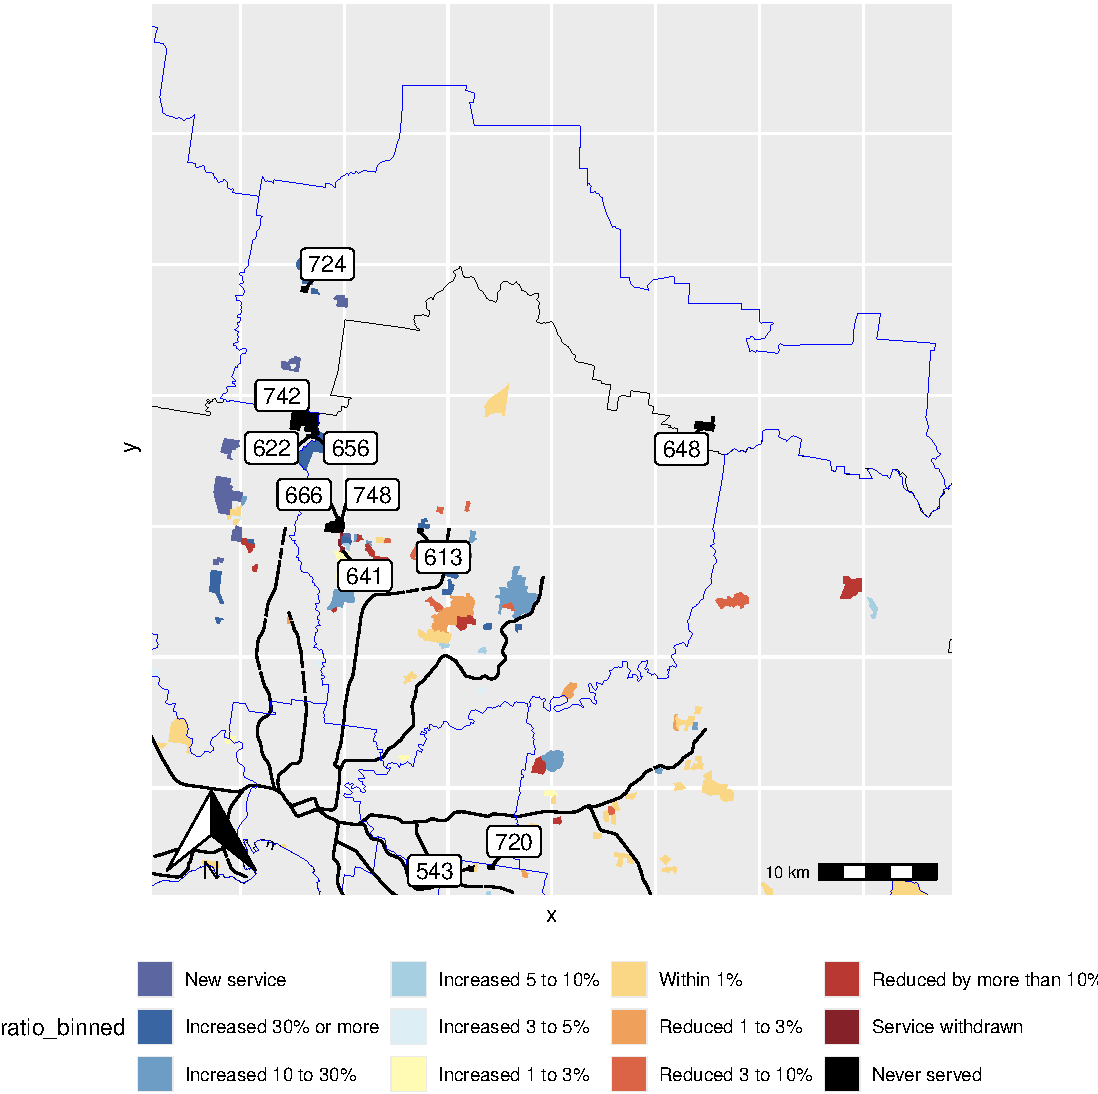
\includegraphics{Leveraging_GTFS_to_assess_transit_supply_Transport_Geography_files/figure-latex/outer_east_changes-1.pdf}
\caption{Greater Melbourne SA1s with Very High transport need and Zero
or Very Low supply in 2021, population by change in SI score 2016 to
2021, across SA4.}
\end{figure}

\subsection{How and why spatial patterns have changed since
2006}\label{how-and-why-spatial-patterns-have-changed-since-2006}

\subsection{Duality criterion}\label{duality-criterion}

Other places

Other time periods

\section{Conclusions}\label{conclusions}

\subsection{Limitations}\label{limitations}

\subsection{Directions for furture
research}\label{directions-for-furture-research}

\section*{References}\label{references}
\addcontentsline{toc}{section}{References}

\section{Appendix}\label{appendix}

\begin{figure}
\centering
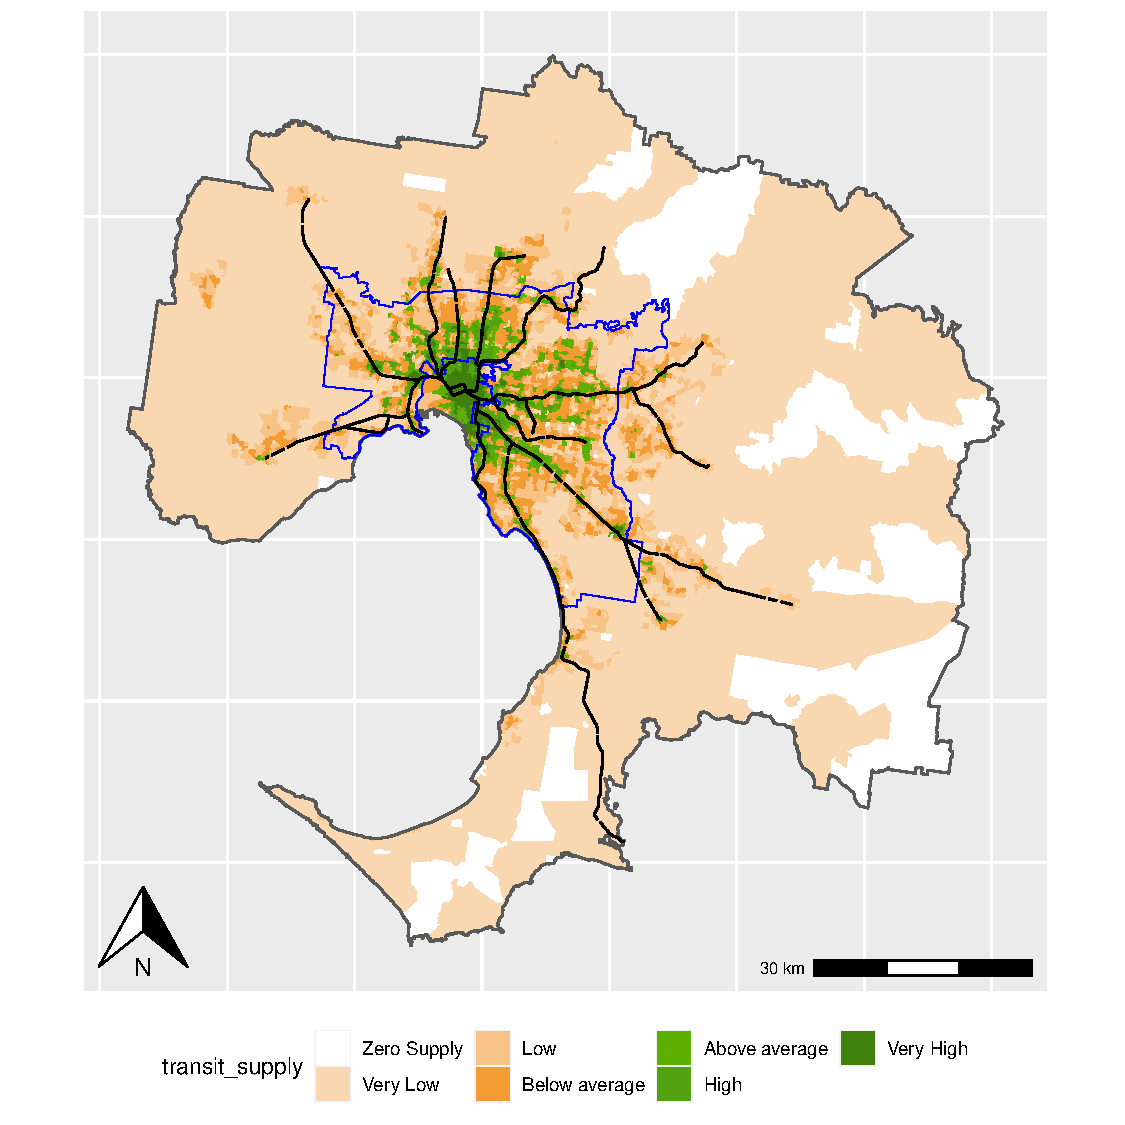
\includegraphics{Leveraging_GTFS_to_assess_transit_supply_Transport_Geography_files/figure-latex/Greater_Melbourne_CCD_2016_appendix-1.pdf}
\caption{Melbourne (2006 extents), Transport Supply by CCD, week
starting the day of the 2016 census, overlayed with inner/middle/outer
suburban boundary (blue) and suburban railway lines (black)}
\end{figure}

\begin{figure}
\centering
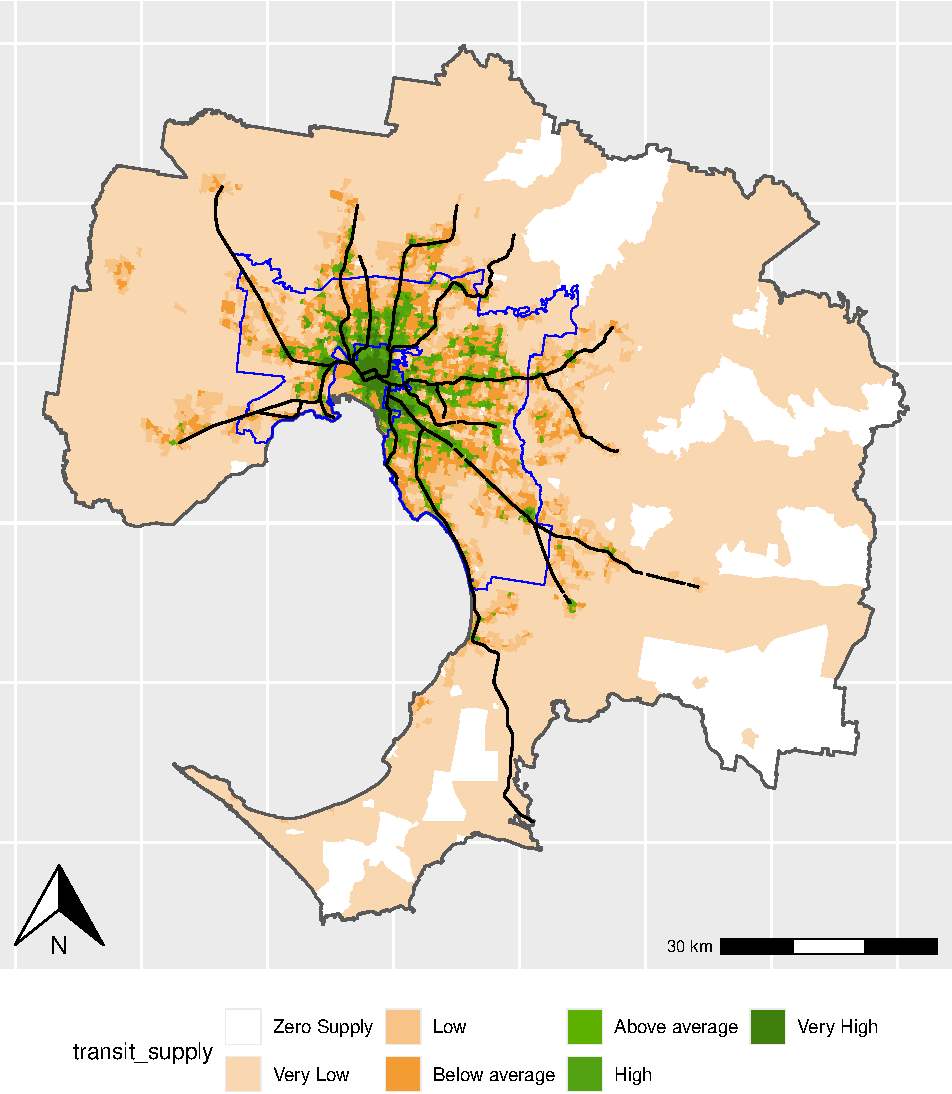
\includegraphics{Leveraging_GTFS_to_assess_transit_supply_Transport_Geography_files/figure-latex/Greater_Melbourne_CCD_2021_appendix-1.pdf}
\caption{Melbourne (2006 extents), Transport Supply by CCD, week
starting the day of the 2021 census, overlayed with inner/middle/outer
suburban boundary (blue) and suburban railway lines (black)}
\end{figure}

Figures \ref{fig:Greater_Melbourne_CCD_2016_appendix} and
\ref{fig:Greater_Melbourne_CCD_2021_appendix} show the distribution of
Transport Supply categories across Melbourne in the weeks of the 2016
censuses, using the same (2006) CCD boundaries\footnote{Note, however,
  that there are some inconsistencies in the CCDs included in
  Metropolitan Melbourne in \citet{currie2010identifying} (5,839) and
  the number included in ABS dataset used for this analysis (6,325).} as
in Figure \ref{fig:Currie_map_SI}. The overall spatial patterns appear
generally similar in 2016 and 2021 as they were in 2006, with higher
levels of transit supply in inner areas and close to most railway lines.
However, clear differences include:

\begin{itemize}
\tightlist
\item
  areas in the outer west (around Melton) that had above average supply
  in 2006 had below average supply in 2016 and 2021.
\item
  some middle south-eastern suburbs along the bay (in the vicinty of
  Black Rock) and outer eastern suburbs (Ferntree Gully) have dropped
  below average, while a small areas in the middle to outer south has
  moved from being below average in 2006 to above average in 2016
  (Kananook, immediately north of Frankston) and 2021 (Kananook and
  Bonbeach).
\item
  there have been suburban railway extensions to the north-west
  (Sunbury) and north-east (to South Morang in 2013 and to Mernda in
  2018). The former involved electrification to incorporate existing
  line segments (already served by country services) into the surburban
  network. Transport Supply to Sunbury, however, appears to still be
  below average, suggesting that not much has changed following the
  shift from service by regional trains to suburban trains. For Mernda
  in contrast, there has been increases in service levels, with some
  areas now having Above Average supply.
\item
  Some areas, away from railway lines, have also shifted from below
  average supply in 2006 to above average supplies in 2016 and 2021,
  including in the middle north-west (Greenvale) and middle to outer
  south east (Narre Warren South).
\item
  Services appear to have been introduced to some outer eastern (east of
  Gembrook), south-eastern (Koo Wee Rup, Lang Lang, Nar Nar Goon,
  Garfield, Bunyip and others) and southern (St Andrews Beach) areas.
\end{itemize}

\begin{figure}
\centering
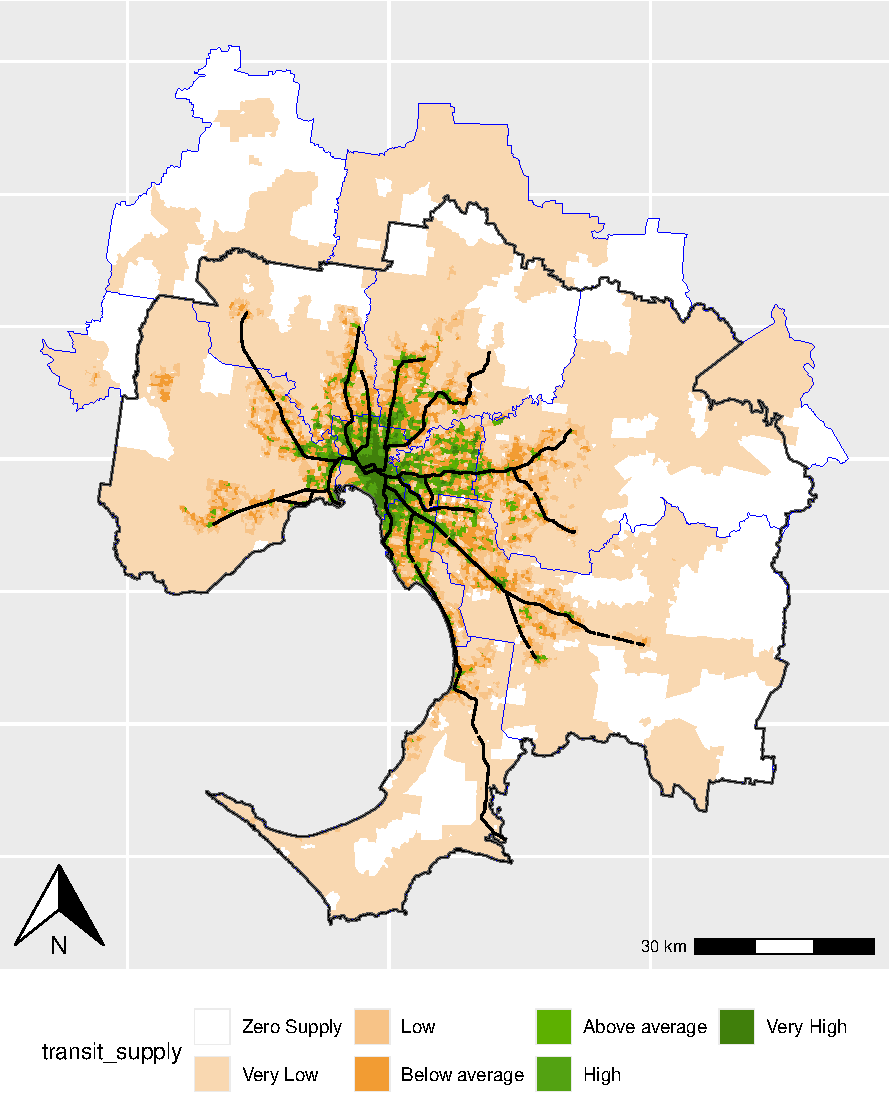
\includegraphics{Leveraging_GTFS_to_assess_transit_supply_Transport_Geography_files/figure-latex/Greater_Melbourne_SA12016_plot_appendix-1.pdf}
\caption{Greater Melbourne, Transit Supply by SA1 for the week starting
the date of the 2016 census, overlayed with: 2006 Greater Melbourne
boundary (black); 2021 SA4 boundaries (blue); and suburban railway lines
(black)}
\end{figure}

\begin{figure}
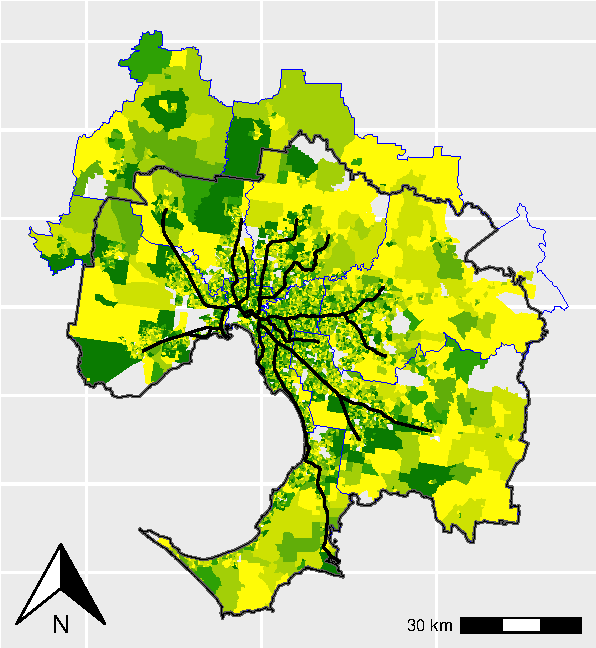
\includegraphics[width=0.9\linewidth]{Leveraging_GTFS_to_assess_transit_supply_Transport_Geography_files/figure-latex/Greater_Melbourne_2016_social_needs_appendix-1} \caption{Distribution of categories of composite social need index scores in 2016 (left) and 2021 (right), overlayed with: 2006 Greater Melbourne boundary (black); middle/outer and inner/middle suburb boundaries (grey); and suburban railway lines (dashed).}\label{fig:Greater_Melbourne_2016_social_needs_appendix}
\end{figure}

Figure \ref{fig:Greater_Melbourne_2016_social_needs_appendix} shows the
spatial patterns of social needs in 2016. Compared to 2021, the spatial
patterns appear similar, with some areas in the north-west (Gisborne)
and south-east (Carrum Downs, Stoney Point) having Very High needs in
both. Some caution may be required in making direct comparisons of many
outer suburbs where residential development has led to the introduction
of new SA1s for the 2021 census. In many areas, including in the
south-west (Werribee), north-west (Romsey), north (Wallan, Beveridge,
Mickleham) and south-east (Clyde North and Beaconsfield South), it
appears there are still Very High transport needs but the spatial area
covered on the map is much smaller due to the redistricting of larger
SA1s into multiple SA1s. That said, it appears that:

\begin{itemize}
\tightlist
\item
  social needs fell in the southern parts of Bacchus Marsh and areas
  around Melton (outer west);
\item
  social needs rose in some outer northern (Lancefield), eastern
  (Gembrook East) and southern (end of the Mornington Penninsula) areas.
\end{itemize}

\begin{figure}
\centering
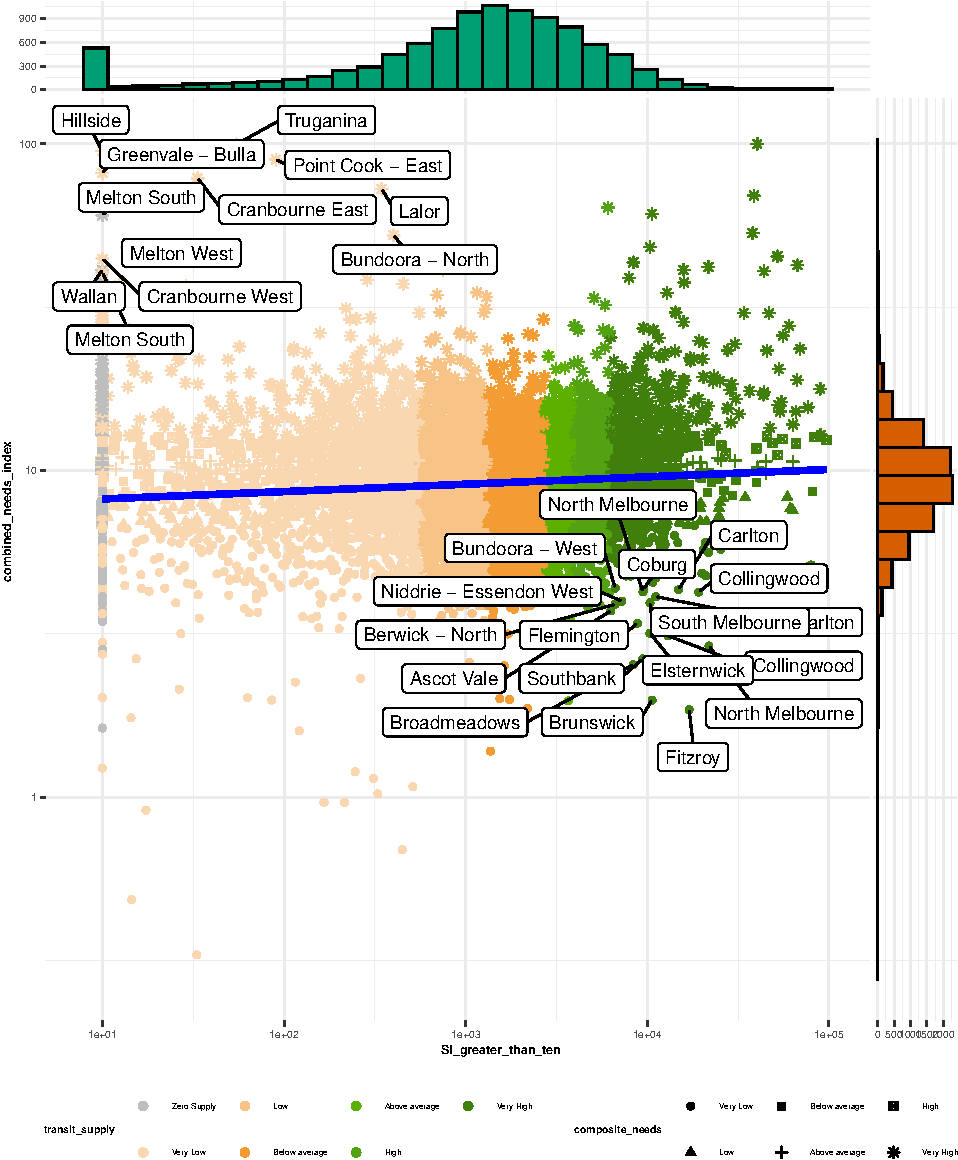
\includegraphics{Leveraging_GTFS_to_assess_transit_supply_Transport_Geography_files/figure-latex/Greater_Melbourne_2016_needs_gap_scatterplot_figure-1.pdf}
\caption{Greater Melbourne 2016, SI and Combined Needs Index scores,
with SI scores \textless{} 10 rounded up to equal 10.}
\end{figure}

\bibliography{References.bib, packages.bib}


\end{document}
